%%%%%%%%%%%%%%%%%%%%%%%%%%%%%%%%%%%%%%%%%%%%%%%%%%%%%%%%%%%%%%%%%%%%%%%
% Universidade Federal de Santa Catarina             
% Biblioteca Universitária                     
%----------------------------------------------------------------------
% Exemplo de utilização da documentclass ufscThesis
%----------------------------------------------------------------------                                                           
% (c)2013 Roberto Simoni (roberto.emc@gmail.com)
%         Carlos R Rocha (cticarlo@gmail.com)
%         Rafael M Casali (rafaelmcasali@yahoo.com.br)
%%%%%%%%%%%%%%%%%%%%%%%%%%%%%%%%%%%%%%%%%%%%%%%%%%%%%%%%%%%%%%%%%%%%%%%
\documentclass{ufscThesis} % Definicao do documentclass ufscThesis	

%----------------------------------------------------------------------
% Pacotes usados especificamente neste documento
\usepackage{graphicx} % Possibilita o uso de figuras e gráficos
\usepackage{color}    % Possibilita o uso de cores no documento
%\usepackage{pdfpages} % Possibilita a inclusão da ficha catalográfica
\usepackage{listings} % Possibilita colocar códigos

\usepackage{caption} % colocar textos em figuras
\usepackage{subfigure}

%\usepackage{hyperref} % colocar hyperlinks no texto

\usepackage{xifthen} % deixa fazer uns if-then-else mutcho loko

\usepackage[brazil]{babel}  % usados para arrumar os caracteres em português
\usepackage[utf8]{inputenx} % 
\usepackage[T1]{fontenc}    %

\usepackage{bibentry} % permite usar o comando nobibliography

\usepackage[newfloat]{minted} % Sintaxe colorida

\usepackage{xparse} % Permite definir umas funções com mais recursos.

\usepackage{amsmath} % Permite usar equation*

\usepackage{mdframed}

%----------------------------------------------------------------------
% comandos de customização dos pacotes
\renewcommand{\thelisting}{\arabic{listing}}
\SetupFloatingEnvironment{listing}{name=Algoritmo,listname={Lista de Algoritmos},within=none}
\captionsetup[listing]{position=above,skip=2pt}
\captionsetup[figure]{position=above,skip=2pt}
\captionsetup[table]{position=above,skip=2pt}

\DeclareFloatingEnvironment[name=Equação,listname={Lista de Equações}]{equacao} % \listof...
\renewcommand{\theequacao}{\arabic{equacao}}
\captionsetup[equacao]{position=above,skip=0pt}

\DeclareFloatingEnvironment[name=Apêndice,listname={Apêndices},within=none]{lstappendix}
%\renewcommand{\thelstappendix}{\arabic{listing}}

\graphicspath{{figuras/}}

%----------------------------------------------------------------------
% Comandos criados pelo usuário
\newcommand{\afazer}[1]{{\color{red}{#1}}} % Para destacar uma parte a ser trabalhada
\newcommand{\ABNTbibliographyname}{REFERÊNCIAS} % Necessário para abnTeX 0.8.2

\newcommand{\figura}[5][Extraido de:]{
\begin{figure}[h!tb]
	\centering
	\caption{#3.}
	\includegraphics[width=#4]{#2.png}
	\ifthenelse{\isempty{#5}}{}{%
		\\ #1 \citeonline{#5}.
	}	
	\label{fig:#2}
\end{figure}
}

\NewDocumentEnvironment{tabela}{mm}
{
	\begin{table}[htb]
		\centering
}
{
		\caption{#2}
		\label{tab:#1}
	\end{table}
}

\newenvironment{algoritmo}[4][]{
\VerbatimEnvironment
\begin{mdframed}[linecolor=black,topline=false,bottomline=false,leftline=false,rightline=false,backgroundcolor=white]
	\captionof{listing}{#3.}
	\label{alg:#2}
	\begin{minted}[mathescape,linenos,numbersep=5pt,gobble=0,frame=lines,framesep=2mm,tabsize=4,fontsize=\footnotesize,breaklines=true,#1]{#4}}{
	\end{minted}
\end{mdframed}
}

%\newenvironment{algoritmo}[4][]{
%	\VerbatimEnvironment
%	\begin{listing}
%		\caption{#3.}
%		\label{alg:#2}
%		\centering
%		\begin{minted}[mathescape,linenos,numbersep=5pt,gobble=0,frame=lines,framesep=2mm,tabsize=4,fontsize=\footnotesize,breaklines=true,#1]{#4}}{
%		\end{minted}
%	\end{listing}
%}

\newenvironment{apendiceAlgoritmo}[4][]{
	\VerbatimEnvironment
	\begin{lstappendix}
		\caption{#3.}
		\label{ape:#2}
		\centering
		\begin{minted}[mathescape,linenos,numbersep=5pt,gobble=0,frame=lines,framesep=2mm,tabsize=4,fontsize=\footnotesize,#1]{#4}}{
		\end{minted}
	\end{lstappendix}
}

\newcommand{\reffig}[1]{Figura \ref{fig:#1}}
\newcommand{\refalg}[1]{Algoritmo \ref{alg:#1}}
\newcommand{\refape}[1]{Apêndice \ref{ape:#1}}
\newcommand{\reftab}[1]{Tabela \ref{tab:#1}}
\newcommand{\refcap}[1]{\footnote{vide tópico \ref{cap:#1}.}}
\newcommand{\reftop}[1]{Seção \ref{cap:#1}}
\newcommand{\refequ}[1]{Equação \ref{equ:#1}}

\newcommand{\criarSigla}[3][]{%
	\ifthenelse{\isempty{#1}}{%
		#2 (#3)\sigla{#3}{#2}%
	}{%
		\emph{#2} (#3)\sigla{#3}{\emph{#2}}\footnote{Traduzido como: #1.}%
	}%
}

\newcommand*\justify{%
	\fontdimen2\font=0.4em% interword space
	\fontdimen3\font=0.2em% interword stretch
	\fontdimen4\font=0.1em% interword shrink
	\fontdimen7\font=0.1em% extra space
	\hyphenchar\font=`\-% allowing hyphenation
}

%----------------------------------------------------------------------


%----------------------------------------------------------------------
% Identificadores do trabalho
% Usados para preencher os elementos pré-textuais
\instituicao[a]{Universidade Federal de Santa Catarina} % Opcional
\departamento[a]{} %TODO departamento de engenharia da computação?
\curso[a]{Universidade Federal de Santa Catarina}
\documento[o]{Trabalho\ de\ Conclusão\ de\ Curso} % [o] para dissertação [a] para tese
\titulo{OpenAutOS}
\subtitulo{Um Sistema Operacional Veícular} % Opcional
\autor{Bruno Fontana Canella}
\grau{Bacharel em Engenharia de Computação}
\local{Araranguá} % Opcional (Florianópolis é o padrão)
\data{04}{Julho}{2017}
\coordenador[Coordenador\\Universidade Federal de Santa Catarina]{Prof. Dr. Anderson Luiz Fernandes Perez}
\orientador[Orientador\\Universidade Federal de Santa Catarina]{Prof. Dr. Anderson Luiz Fernandes Perez}
%\coorientador[Coorientador\\Universidade ...]{Prof. Dr.}

\numerodemembrosnabanca{2} % Isso decide se haverá uma folha adicional
\orientadornabanca{não} % Se faz parte da banca definir como sim
\coorientadornabanca{não} % Se faz parte da banca definir como sim
\bancaMembroA{Prof. Dr. Anderson Luiz Fernandes Perez\\Universidade Federal de Santa Catarina} %Nome do presidente da banca
\bancaMembroB{Prof. Dr. Fábio Rodrigues De La Rocha\\Universidade Federal de Santa Catarina}      % Nome do membro da Banca
\bancaMembroC{Prof. Dr. Marcelo Daniel Berejuck\\Universidade ...}     % Nome do membro da Banca
%\bancaMembroD{Quarto membro\\Universidade ...}       % Nome do membro da Banca
%\bancaMembroE{Quinto membro\\Universidade ...}       % Nome do membro da Banca
%\bancaMembroF{Sexto membro\\Universidade ...}        % Nome do membro da Banca
%\bancaMembroG{Sétimo membro\\Universidade ...}       % Nome do membro da Banca

\dedicatoria{Dedico este trabalho ao meu orientador, Anderson Luiz Fernandes Perez, a todos os amigos que fiz durante meu período de graduação na UFSC Araranguá, incluindo alunos, docentes e funcionários em geral, e a minha família.}

\agradecimento{Gostaria de começar prestando meus agradecimentos a dois alunos e amigos do curso de Engenharia da Computação da UFSC Araranguá: Alan Kunz Cechinel e Thiago Dal Pont, sem os quais minha jornada até a entrega do TCC e graduação teriam sido bem mais árduas e demoradas. Por todas as tarde me ensinando, pacientemente, os conteúdos de difícil compreensão do curso, bem como nas ajudas nos trabalhos e pela amizade em geral, deixo aqui o meu muito obrigado.

Gostaria também de agradecer formalmente ao professor Anderson Luiz Fernandes Perez por todo o esforço, compreensão e incentivo na produção deste trabalho de conclusão de curso. Não fosse pelo seu encorajamento, este trabalho seria algo bem mais simples e menos desafiador do que meu esforço e dedicação poderiam alcançar. 

A minha família, que em nenhum momento duvidou das minhas capacidades e que sempre acreditou que eu terminaria o TCC sem reprovar nenhuma vez, dessa vez, e que também não ficou pegando no meu pé por causa do TCC da faculdade passada.

A todas as pessoas do Laboratório de Automação e Robótica Móvel (LARM), do qual fiz parte, e que conseguiu sempre manter uma atmosfera acolhedora e focada no aprendizado e desenvolvimento do campus e do curso.

E por fim, mas não menos importante, a todas as amizades que eu fiz durante este período da minha vida aqui na UFSC Araranguá.}

\epigrafe{Escrever um TCC é que nem fazer estrada. Depois que tá feita a base é só passar asfalto.}{(Anderson, 2016)}
% "knowledge is power, and I like power" - Cobra Bubbles - Lilo & Stitch

\textoResumo {
	Com a quantidade cada vez maior de dispositivos eletrônicos sendo agregados aos veículos automotivos e, por consequência, de ECUs para gerência-los, tornou-se necessário a criação de padrões de comportamento e comunicação para estas centrais, afim de garantir que diferentes fabricantes pudessem desenvolver soluções veiculares intercambiáveis, sem que se preocupassem com estes pontos de integração.
	Como resultado da padronização surgiram padrões tanto para o desenvolvimento de hardware quanto para o de software, sendo que atualmente o padrão AUTOSAR é o mais utilizado pela indústria automotiva.
	Devido a maioria das soluções existentes hoje no mercado, que respeitam este padrão, serem proprietárias, este trabalho propõe o desenvolvimento de um sistema operacional de qualidade comercial e código aberto, baseado nestas mesmas normas, e que possa ser utilizada como referencia de aprendizagem e, até mesmo, como uma alternativa para a programação de ECUs automotivas.}
\palavrasChave {Automação Veicular, Sistema Operacional Embarcado, AUTOSAR, OpenAUTOS.}

\textAbstract {
	Due to the increasing amount of electronic devices being added to automotive vehicles and, by consequence, of ECUs to manage them, it became necessary to create behavioral and communication standards for these centrals in order to ensure that different manufacturers could develop interchangeable vehicle solutions without having to worry about these points of integration.
	As a result of standardization, standards have emerged for both hardware and software development, and today AUTOSAR standard is the one most used by the automotive industry.	
	Due to the majority of the existing solutions in the market that respect this standard being proprietary, this thesis proposes the development of a commercial quality and open source operating system, based on those same standards, and that can be used as a learning reference and even as an alternative in the development of automotive ECUs.}
\keywords {Vehicle Automation, Embedded Operating Systems, AUTOSAR, OpenAUTOS.}

%----------------------------------------------------------------------
% Início do documento                                
\begin{document}
%--------------------------------------------------------
% Elementos pré-textuais
\capa  
%\folhaderosto[comficha] % Se nao quiser imprimir a ficha, é só não usar o parâmetro

\begin{titlepage}
	\vfill
	\begin{center}
		%{\large \ABNTautordata} \\[5cm]
		\ABNTautordata \\[5cm]
		
		\tituloformat{\ABNTtitulodata}: \\
		\tituloformat{\subtitulodata} \\[1cm]
		
		\hspace{.45\textwidth} % posicionando a minipage
		\begin{minipage}{.5\textwidth}
			\begin{espacosimples}
				
				Trabalho de Conclusão de Curso submetido à \ABNTinstituicaodata,
				como parte dos requisitos necessários para a obtenção do Grau de
				Bacharel em Engenharia de Computação.
				
				Orientador: Prof. Anderson Luiz Fernandes Perez, Dr.
			\end{espacosimples}
		\end{minipage}
		\vfill \localformat \ABNTlocaldata, \mesdata\ de \anodata.
	\end{center}
	\vspace{1cm}
\end{titlepage}

%\folhaaprovacao
\paginadedicatoria
\paginaagradecimento
\paginaepigrafe
\paginaresumo
\paginaabstract
%\pretextuais % Substitui todos os elementos pre-textuais acima
\listadefiguras % as listas dependem da necessidade do usuário
\listadetabelas 
\listadeabreviaturas
%\listadesimbolos
%\listoflisting
{%
	\renewcommand{\figurename}{}%
	\let\oldnumberline\numberline%
	\renewcommand{\numberline}{\listingname~\oldnumberline}%
	\listoflisting%
}
%{%
%	\renewcommand{\figurename}{}%
%	\listoflstappendix%
%}
\sumario

%--------------------------------------------------------
% Simbolos e Abreviaturas
\abreviatura{RAM}{\emph{Random Access Memory}}
\abreviatura{ROM}{\emph{Read-Only Memory}}
%--------------------------------------------------------
% Elementos textuais

\chapter{Introdução}

Desde seu surgimento, popularização e evolução até os dias atuais, os veículos automotivos aumentaram em muito a sua complexidade, a ponto de que apenas o conhecimento mecânico do veículo não é mais suficiente. A quantidade de componentes eletrônicos presentes nos veículos automotivos aumentou consideravelmente passando, inclusive, a substituir sistemas puramente mecânicos. Fatores que alavancaram estas mudanças incluem o barateamento, miniaturização e popularização dos componentes eletrônicos.

Com o propósito de padronizar e, assim, facilitar o desenvolvimento e intercambialidade de auto-peças por terceiros, as principais montadoras e fabricantes de veículos entraram em um consenso e estipularam um padrão de normas de desenvolvimento para veículos automotivos, chamada de \emph{AUTOSAR}, a qual se encontra em sua quarta revisão.

Para gerenciar os diversos módulos eletrônicos agora presentes em um veículo, bem como garantir a interoperabilidade deles, foi criada uma norma referente ao desenvolvimento de sistemas operacionais. Esta norma visa o estabelecimento de padrões para o funcionamento, comunicação e especificações do sistema, sem sacrificar a liberdade criativa de desenvolvimento do sistema, como a seleção de hardwares e implementação de algoritmos.

%Um dos padrões que surgiu para auxiliar nesta integração foi referente ao desenvolvimento de sistemas operacionais, responsável por gerenciar todos os recursos diretamente relacionados ao funcionamento do veículo. Esta norma visa o estabelecimento de padrões para o funcionamento, comunicação e especificações do sistema, sem sacrificar a liberdade criativa de desenvolvimento do sistema, como a seleção de hardwares e implementação de algoritmos.

\section{Justificativa e Motivação}

A maioria das soluções em \emph{SO}s automotivos são exclusivamente comerciais e de código privado. Embora existam soluções de código aberto para sistemas embarcados, não existe, na atualidade, um \emph{SO} de código aberto homologado nos padrões do \emph{AUTOSAR}. O projeto que mais chega próximo deste cenário é o \emph{Trampoline}, que se encontra em fase de homologação da norma.

Visando a criação de um \emph{SO} embarcado, para uso em veículos populares, e que mantivesse um padrão de código aberto, surgiu a idealização do \emph{OpenAUTOS}. Com o desenvolvimento do \emph{OpenAUTOS} é desejado conseguir um modelo de SO nacional, com componentes e tecnologia disponíveis de fácil acesso, proporcionando também contribuir com a própria comunidade acadêmica.

\section{OBJETIVOS}

Esta seção apresenta o objetivo geral e os objetivos específicos deste trabalho.

\subsection{Geral}

Desenvolver um sistema operacional embarcado de código aberto que atenda as normas estabelecidas pelo padrão \emph{AUTOSAR}.

\subsection{Específicos}
\begin{enumerate}
	\item Levantar o estado da arte com respeito a algoritmos para sistemas operacionais embarcados;
	\item Estudar padrões de sistemas automotivos;
	\item Levantar os requisitos para implementação de um \emph{SO} de acordo com a norma \emph{AUTOSAR};
	\item Estabelecer um projeto de código aberto em um repositório online;
	\item Documentar o código do projeto;
	\item Criar um modelo físico que utilize o \emph{SO} desenvolvido;
	\item Realizar a instalação do \emph{SO} em um veículo automotivo real;
\end{enumerate}

\section{Organização do trabalho}

Este trabalho está dividido em 4 capítulos, contando com a introdução.

O \textbf{Capítulo 2} apresentará os domínios eletrônicos de funcionamento em veículos, seus meios de comunicação, unidades de controle e engenharia de software automotivo.

O \textbf{Capítulo 3} abordará os principais conceitos sobre sistemas operacionais. Ao final do capítulo serão relatados alguns estudos de caso a respeito de sistemas operacionais embarcados com foco para a automação veicular.

O \textbf{Capítulo 4} apresentará a proposta do SO \emph{OpenAUTOS}, destacando as escolhas e a arquitetura adotada.


\chapter{Automação Veicular}
\label{cap:automacao_veicular}

%Breve introdução
%Tipos de Automação Veicular
%Padrões para o Desenvolvimento de Software para Automação Veicular
%Sistemas Operacionais Embarcados para Automação Veicular


%- Introdução
%- Definição (o que é, quais os itens que são relevantes: chassi,
%carroceria, power train, infotainement, ....)
%- Descrever cada item da automação veicular
%- Falar sobre ECUS
%- Escrever sobre Engenharia de Software para Automação Veicular
%- Descrever os padrões AUTOSAR e OSEK/VDX

\chapter{Sistemas Operacionais Embarcados}

Neste capítulo são abordados os principais conceitos sobre sistemas operacionais. Ao final do capítulo são relatados alguns estudos de caso a respeito de sistemas operacionais embarcados com foco para a automação veicular.

\section{Sistemas Operacionais}

O objetivo de um SO é o de gerenciar os recursos de um sistema computacional, tornando transparente seu funcionamento para o usuário final. O SO é o componente de software que faz a união e abstração dos recursos de hardware e os oferece de maneira simplifica para as aplicações utilizadas pelo usuário final. A \reffig{cap3_os_parts} ilustra a visão abstrata de um SO, ou seja, o SO como um provedor de serviços para as aplicações de usuários.

\figura[Adaptado de:]{cap3_os_parts}{Visão geral da integração do SO com o sistema computacional}{4cm}{osc9}

Segundo \citeonline{osc9}, um SO pode oferecer um número variável de serviços. Os serviços do SO que estão sempre presentes na memória principal fazem parte do kernel, que é descrito na \reftop{os_kernel}. 

Para que os aplicativos tenham acesso aos serviços oferecidos sem que haja um comprometimento de sua integridade, o SO oferece rotinas de acesso aos serviços. A quantidade de serviços varia conforme implementação do SO, sendo o mínimo oferecido as operações de gerenciamento de processos, memória e \criarSigla{Entrada e Saída}{E/S}. A \reffig{cap3_os_services} apresenta uma hierarquia de chamada dos serviços do SO.

\figura[Adaptado de:]{cap3_os_services}{Serviços de um SO}{6cm}{osc9}

\subsection{Kernel}
\label{cap:os_kernel}

\citeonline{linfo} define o \emph{kernel} como sendo o programa que constitui o núcleo central de um sistema operacional. Ele é responsável por fazer o gerenciamento dos recursos de hardware bem como sua abstração para os aplicativos do usuário. A \reffig{cap3_os_kernel_layers} ilustra onde se encontra a camada de abstração do \emph{kernel}.

\figura{cap3_os_kernel_layers}{Posição conceitual do \emph{kernel}}{3.5cm}{minix}

Em sistemas computacionais convencionais, o \emph{kernel} é a primeira parte do SO a ser carregada na memória durante o processo de inicialização. Uma vez carregado, o \emph{kernel} permanece na memória principal do sistema até que o mesmo seja desligado. Para \criarSigla{Sistemas Operacionais Embarcados}{SOE}, o \emph{kernel} sempre está presente na memória de programa. Após uma instrução de \emph{reset}, é sempre o primeiro código a ser executado. A \reffig{cap3_os_kernel_memory} ilustra ambos os modelos.

\figura[Adaptado de:]{cap3_os_kernel_memory}{Posição do \emph{kernel} na memória}{7cm}{qingli}

\section{Estrutura dos Sistemas Operacionais}

Independente dos serviços oferecidos, um SO pode ser separado em quatro serviços principais: gerenciamento de processos, de memória, de entrada e saída de dados e sistemas de arquivos.

\subsection{Gerenciamento de Processos}

O gerenciamento de processos consiste no tratamento de interrupções, controle de tarefas e acesso a recursos do sistema, de uma maneira que nenhum dos processos entre em conflito ou pare sua execução permanentemente, que não de maneira espontânea.

A quantidade de elementos que compõem um SO varia conforme implementação, mas geralmente incluem: tarefas, semáforos, filas de mensagem, entre outras.

\subsubsection{Tarefas}

Em um SO convencional, cada programa que é executado no computador toma a forma de um processo, que pode ser definido como uma atividade que possui sua própria pilha, área de memória privada, e que pode alocar memória dinamicamente conforme a necessidade, muitas vezes sem precisar se preocupar com a falta do recurso. Mais programas podem ser adicionados a qualquer momento em um SO para computadores.

Em sistemas embarcados, o conceito de processo é substituído pelo de \emph{tarefas}, onde a principal diferença está no fato de que todas as tarefas ja estão definidas no momento em que o SO inicia. Para criar novos tipos de tarefas é necessário parar o SO e adicioná-las manualmente.

Uma tarefa pode assumir um número de estados pré-determinado, os quais variam conforme o SO utilizado, mas geralmente incluem os estados presentes na \reffig{cap3_process_tasks_states}, conforme visto em \citeonline{osc9}. Estes estados podem ser descritos como:

\begin{itemize}
	\item \textbf{Iniciando}: etapa inicial, onde são executadas instruções de preparo para a tarefa;
	\item \textbf{Pronto}: indica que a tarefa está pronta para ser executada, mas que ela não é a tarefa ativa, no momento;
	\item \textbf{Executando}: estado da tarefa que está em execução no SO;
	\item \textbf{Bloqueado}: a tarefa está aguardado a ocorrência de algum evento externo para que ela possa voltar a executar;
	\item \textbf{Finalizado}: a tarefa libera recursos alocados, antes de ser encerrada definitivamente.
\end{itemize}

\figura{cap3_process_tasks_states}{Estados de uma tarefa}{8cm}{osc9}

\paragraph{Fibras}

Uma variante das tarefas são as fibras, que são threads de execução leves e não-preemptivas, normalmente utilizadas para executar porções de código responsáveis pelos drivers de dispositivos e outras atividades consideradas de desempenho crítico \cite{rocket}.

\subsubsection{Escalonadores de Tarefas}

O escalonamento de tarefas surgiu para permitir que mais de uma tarefa fique em execução no processador, sem que ela tenha que concluir seu funcionamento para que isso aconteça. Na prática, isso gera uma situação na qual várias tarefas aparentam estar em execução ao mesmo tempo, em arquiteturas com um único processador.

\citeonline{minix} descreve alguns tipos de algoritmos para escalonamento. Serão apresentados aqui apenas os escalonadores mais utilizados em RTOSes, sendo eles Round Robin, Prioridade e Prioridade com Round Robin.

\paragraph{Escalonador Round Robin}

No escalonador Round Robin, uma tarefa permanece em execução apenas por um valor $\Delta T$ de tempo, geralmente na casa dos $us$, após a qual ela é movida para o estado de \emph{Pronto}, colocando a próxima tarefa na fila em execução, conforme ilustrado na \reffig{cap3_process_scheduler_rr}.

\figura{cap3_process_scheduler_rr}{Diagrama esquemático de funcionamento do algoritmo de escalonamento Round Robin}{8cm}{minix}

\paragraph{Escalonador por Prioridade}

Neste tipo de escalonador, a tarefa é associada a um atributo numérico, o qual indica o nível de sua prioridade. A tarefa de mais alta prioridade que não estiver bloqueada será sempre a que estará em execução no SO. Ela permanece em execução até que se auto-bloquei, seja por uma rotina de \emph{delay}, por tentar acessar um recurso indisponível no momento, ou ainda porque uma tarefa de maior prioridade ficou disponível.

A \reffig{cap3_process_scheduler_prio} apresenta um escalonador por prioridade em dois momentos. No momento \emph{(a)}, a tarefa em execução chama uma rotina que faz seu auto-bloqueio. No instante de tempo \emph{(b)}, a tarefa em execução passa a ser a próxima tarefa de prioridade mais alta, disponível naquele momento.

\figura{cap3_process_scheduler_prio}{Diagrama esquemático de funcionamento do algoritmo de escalonamento baseado em prioridade}{6cm}{minix}

\paragraph{Escalonador por Prioridade com Round Robin}

Faz uma junção dos dois tipos de escalonadores apresentados anteriormente. Funciona da mesma maneira que o escalonador de prioridades, exceto que agora é possível ter mais de uma tarefa com o mesmo nível de prioridade. Quanto este cenário ocorrer, as tarefas de mesma prioridade ficarão alternando a posição de \emph{em execução}, através do algoritmo Round Robin.

A \reffig{cap3_process_scheduler_rr_prio} apresenta um exemplo deste escalonador, onde após um intervalo de tempo $\Delta T$, ocorre a troca de contexto para a próxima tarefa de mesma prioridade que não se encontra bloqueada.

\figura{cap3_process_scheduler_rr_prio}{Diagrama esquemático de funcionamento do algoritmo de escalonamento baseado em prioridade com Round Robin}{5cm}{minix}

\subsubsection{Semáforos}

Múltiplas tarefas em execução concorrente devem ser capazes de sincronizar suas ações e coordenar o acesso mutuamente exclusivo a recursos compartilhados. Para atender a estes requisitos, o SO pode prover um objeto chamado semáforo.

Um semáforo funciona como uma espécie de chave que permite a uma tarefa acessar algum tipo de operação ou recurso. Se a tarefa puder adquirir um semáforo, ela poderá continuar sua execução normalmente. Do contrário, a tarefa poderá ser bloqueada até que o recurso esteja disponível novamente.

Segundo \citeonline{minix}, existem semáforos de contagem, binários e de exclusão mútua. Semáforos de contagem e binários apresentam comportamentos similares, tendo como única diferença que um semáforo binário possui seu valor máximo igual a $1$. Um diagrama de atividades, demostrando o funcionamento de um semáforo pode ser visto na \reffig{cap3_process_semaphore}.

\figura[Adaptado de:]{cap3_process_semaphore}{Transição de Estados para Semáforos de Contagem}{\textwidth}{qingli}

\paragraph{Mutex}

O semáforo do tipo \emph{mutex} atende a um caso especial do semáforo binário, chamado de semáforo de exclusão mútua ou \emph{mutex}. Um \emph{mutex} pode suportar propriedades de posse, trava recursiva, deleção segura de tarefas, dentre outros serviços, afim de evitar problemas inerentes a exclusão mútua.

\subsubsection{Filas de Mensagens}

Uma fila de mensagens é um objeto através do qual as tarefas e \criarSigla[Rotina de Serviço para Interrupções]{Interrupt Service Routine}{ISR} enviam e recebem mensagens para comunicação e sincronização de dados. Elas armazenam temporariamente as mensagem do remetente até que o destinatário esteja pronto para recebe-las. Isto garante o desacoplamento entre a tarefa emissora e receptora.

Uma fila de mensagens é composta por objetos chamados de \emph{elementos}, dos quais cada um pode armazenar uma única mensagem, a qual pode estar vazia. O número total de elementos na fila equivale ao seu comprimento. A \reffig{cap3_process_messages_queues} apresenta um esquema para as filas de mensagem.

\figura[Adaptado de:]{cap3_process_messages_queues}{Diagrama esquemático do funcionamento de uma fila de mensagens.}{\textwidth}{qingli}

\subsubsection{Sinais}

Um sinal é uma interrupção gerada por software, a qual dispara quando ocorre um evento. Assim como numa interrupção, um sinal faz com que o processo em execução seja interrompido para executar uma outra rotina assíncrona.

Na essência, os sinais notificam as tarefas de eventos que ocorreram durante a execução de outras tarefas ou ISRs. Assim como as interrupções, estes eventos são assíncronos para a tarefa notificada e não ocorrem em nenhum ponto pré-determinado durante sua execução. A principal diferença entre uma interrupção e um sinal é que o primeiro é gerado por hardware, como quando um pino de um microcontrolador passa de $0V$ para $5V$, enquanto o último é gerado por software.

Quando há a chegada de um sinal, a tarefa desvia de seu fluxo normal de execução, e a \criarSigla[Rotina de Sinal Assíncrona]{Asynchronous Signal Routine}{ASR} correspondente é invocada, conforme ilustrado na \reffig{cap3_process_signals}.

\figura[Adaptado de:]{cap3_process_signals}{Tratamento de sinal em uma tarefa}{8cm}{qingli}

\subsection{Gerenciamento de Memória}

Em muitos dos sistemas embarcados (tais como celulares, câmeras digitais, \emph{tablets}) há um número limitado de aplicações (tarefas) que  podem estar em execução em um dado momento. Parte do motivo é que estes dispositivos apresentam um quantidade limitada de memória física. Dispositivos maiores, como roteadores de rede, possuem uma maior quantidade de memória física instalada, mas também fazem maior uso dela e precisam de um gerenciamento ainda maior deste recurso.

Independente do tipo de sistema embarcado, os requisitos comuns a sistemas de gerenciamento de memória são a mínima fragmentação, mínima sobrecarga em operações de gerenciamento e tempos de alocação determinísticos.

\subsubsection{Alocação Dinâmica de Memória}

O código do programa, seus dados e a pilha do sistema ocupam a memória física do sistema embarcado, uma vez carregados e inicializados. A memória restante é utilizada para alocação dinâmica pelo RTOS ou pelo \emph{kernel}. Esta área recebe o nome de \emph{heap}\footnote{Tanto a \emph{Stack} quanto a \emph{Heap} são áreas de memória para um programa. A diferença entre elas é que a sua alocação é, respectivamente, estática e dinâmica}.

Um gerenciador de memória mantém informações sobre a \emph{heap} em uma área reservada, chamada de bloco de controle. Informações típicas sobre o controle incluem:

\begin{itemize}
	\item O endereço inicial do bloco de memória física utilizado para alocação dinâmica;
	\item O tamanho total de memória disponível;
	\item A tabela de alocações, a qual indica quais áreas da memória estão em uso, quais estão vagas e o tamanho de cada região que ainda está livre.
\end{itemize}

Um sistema de memória deve ser capaz de executar eficientemente as seguintes operações:

\begin{itemize}
	\item Determinar se há um bloco livre que comporta a alocação requisitada;
	\item Manter as informações internas atualizadas;
	\item Mesclar um ou mais blocos, assim que estes forem liberados.
\end{itemize}

A estrutura da tabela de alocação é a chave para um gerenciamento de memória eficaz. Esta estrutura gera um \emph{overhead}, já que ocupa espaço de memória que, outrora, poderia ser utilizado para armazenar dados dos programas. Minimizar a tabela de alocações e maximizar o desempenho das operações anteriores é um dos principais desafios no gerenciamento de memórias.

\subsection{Subsistemas de Entrada/Saída}

Em sistemas embarcados, um sistema de entrada/saída é a combinação dos dispositivos de E/S com os \emph{drivers} de dispositivos associados e subsistemas de E/S.

O propósito de um subsistema de E/S é o de esconder do \emph{kernel} as informações especificas de um dispositivo, assim como do desenvolvedor de aplicações, e prover uma método de acesso uniforme aos periféricos de E/S do sistema embarcado.

A \reffig{cap3_io_layers} ilustra o subsistema de E/S em relação ao resto do sistema em um modelo de camadas de software. Conforme indicado, cada camada descendente agrega mais informações à arquitetura necessária para gerenciar um dado dispositivo.

\figura[Adaptado de:]{cap3_io_layers}{Subsistema de E/S e o modelo por camadas}{7cm}{minix}

\subsubsection{Camada de Abstração}

Cada dispositivo de E/S pode oferecer um conjunto específico de interfaces de programação para os aplicativos. Este arranjo requer que cada aplicativo esteja ciente da natureza do dispositivo de E/S subjacente, incluindo as restrições impostas pelo dispositivo. O conjunto da \criarSigla[Interface de Programação de Aplicação]{Application Programming Interface}{API} é específico à implementação, o que torna difícil a portabilidade das aplicações utilizando esta API. Para reduzir esta dependência, é implementado no sistema embarcado um subsistema de E/S, a qual atua como uma camada de abstração.

Esta camada de abstração define um conjunto padrão de funções para operações de entrada e saída, de forma a esconder as peculiaridades dos dispositivos da aplicação. Todos os \emph{drivers} de E/S passam a se conformar e a suportar este conjunto de funções, já que o objetivo é o de prover uma camada uniforme de E/S para as aplicações. 

Para se alcançar estas operações de E/S uniformemente no nível de aplicação, os seguintes procedimentos devem ser seguidos:

\begin{enumerate}
	\item Definir o conjunto de APIs do subsistema de E/S;
	\item Implementar cada função do conjunto para o driver do dispositivo;
	\item Exportar este conjunto de funções do driver do dispositivo para o subsistema de E/S;
	\item Encarregar ao driver do dispositivo o prepara do mesmo para uso;
	\item Carregar o dispositivo pelo driver do mesmo e informar o subsistema de E/S.
\end{enumerate}

A \reffig{cap3_io_abstraction} ilustra como a camada de E/S abstrai o dispositivo de hardware, garantindo a flexibilidade do sistema.

\figura[Adaptado de:]{cap3_io_abstraction}{Camada de abstração entre o aplicativo e o dispositivo}{\textwidth}{qingli}

\subsection{Sistemas de Arquivos}

Segundo \citeonline{mos4}, um arquivo é uma coleção nomeada de informações relacionadas que são gravadas em uma unidade secundária e persistente de armazenamento. Pela perspectiva do usuário, dados não podem ser salvos em uma unidade secundária, senão pela alocação de um arquivo nela.

Os arquivos são utilizados para guardar informações referentes a dados ou programas. Arquivos de dados podem ser numéricos, alfabéticos, alfanuméricos ou binários. Eles podem também ser estruturados ou não. De maneira geral, um arquivo é uma sequência de bits, no qual o significado varia conforme o criador e usuário do arquivo.

Existem diversos componentes capazes de persistirem estes dados, sendo alguns deles discos e fitas magnéticas, \emph{flash cards} e \emph{Compact Disks}. Para que que o sistema computacional possa utilizar estes dispositivos, o SO deve abstrair as propriedades físicas dos dispositivos de armazenagem e definir uma unidade lógica de armazenagem, capaz de armazenar e localizar facilmente os dados em forma de arquivos.

Um sistema de arquivos provê os meios para organizar os dados, de forma que eles possam ser armazenados, resgatados e atualizados, além de gerenciar o espaço disponível no dispositivo que o contém. Um sistema de arquivos organiza os dados de maneira eficiente e é otimizado para características específicas de um dispositivo \cite{file_system}.

Internamente, um sistema de arquivos funciona de maneira similar a alocação dinâmica da memória principal, onde o sistema armazena informações adicionais sobre a área de dados, como seu tamanho e ponto de origem no dispositivo. Contudo, um sistema de arquivo oferece mais níveis de organização, afim de facilitar o encontro de informações posteriormente, como diretórios, ou ainda controle de permissões, para limitar o acesso de usuários. A \reffig{cap3_fs_directory} apresenta um modelo de organização de diretórios com controle de permissão.

\figura[Adaptado de:]{cap3_fs_directory}{Modelo em árvore de diretórios por usuário}{7cm}{minix}

%A \reftab{fs_sample} apresenta algumas das características de sistemas de arquivos populares. \citeonline{filebenchmark4} contém um estudo mais detalhado de comparação entre sistemas de arquivos.
%
%\begin{tabela}{fs_sample}{Sistemas de Arquivos}
%	\begin{tabular}{|c|c|c|c|}
%		\hline 
%		Sistema de Arquivo & FAT32 & NTFS & ext4 \\ 
%		\hline \hline
%		Plataformas & Muitas & Windows & Linux \\ 
%		\hline 
%		Nome Máximo de Arquivo & 255 bytes & 255 bytes & 255 bytes \\ 
%		\hline 
%		Tamanho Máximo de Caminho & - & 32767 caract. & - \\ 
%		\hline 
%		Tamanho Máximo de Arquivo & 4 Gb & 16 EiB & 16 TiB \\ 
%		\hline 
%		Armazena o Dono do Arquivo & Não & Sim & Sim \\ 
%		\hline 
%		Permissões Posix & Não & Sim & Sim \\ 
%		\hline 
%	\end{tabular}
%\end{tabela}

\section{Sistemas Embarcados}

Um sistema embarcado é um sistema computacional cujo propósito é bem definido e específico. Ele é geralmente conceituado para atender a uma situação particular, com hardware bem definido e, muitas vezes, imutável.

Diferente de um sistema computacional convencional, como os \emph{Desktops} e \emph{Laptops}, um sistema embarcado possuí recursos de hardware bem mais restritos. Por ser projetado para um propósito específico, o mesmo muitas vezes não requer tecnologia de ponta para executar sua tarefa, o que permite a criação de sistemas de baixo custo.

Um sistema embarcado pode ser composto, por exemplo, de sensores e atuadores, bem como uma central de processamento. Em veículos, um exemplo equivalente seria o dos sensores e atuadores para travamento das portas, bem como a central eletrônica responsável por sua operação. A \reffig{cap3_embedded_systems} ilustra diversos sistemas embarcados presentes em um automóvel.

\figura{cap3_embedded_systems}{Sistemas embarcados em um veículo}{\textwidth}{embedded_systems}

\section{Sistemas de Tempo-Real}

Segundo \citeonline{qingli}, uma aplicação de tempo-real é aquela que é composta por múltiplas tarefas independentes em execução, as quais competem pelo tempo de processamento em um processador.

Um sistema de tempo-real pode ser definido como um sistema que responde a eventos externos em tempo hábil. Ou seja, onde o tempo de resposta é uma garantia do sistema. A \reffig{cap3_rtos_constraint} ilustra o conceito de sistema de tempo real, onde independente da entrada, há um tempo limite de resposta, o qual deverá sempre ser respeitado.

\figura[Adaptado de:]{cap3_rtos_constraint}{Resposta em Tempo-Real}{\textwidth}{qingli}

Uma restrição temporal pode ser rígida ou flexível. Restrições rígidas causam uma falha do sistema quando não respeitadas, geralmente causando danos físicos ao equipamento e possível risco humano. Um sistema de restrição flexível não sofre consequências tão graves quando o mesmo falha, mas ainda assim pode causar invalidação do sistema ou de processos. Um veículo possui diversos sistemas embarcados, muitos dos quais possuem restrições temporais, tanto rígidas quanto flexíveis.

\section{Estudos de Caso}

A seguir são apresentados alguns estudos de casos sobre sistemas operacionais embarcados já existentes no mercado.

\subsection{FreeRTOS}

Conforme \citeonline{FreeRTOS:HOME}, o FreeRTOS é uma solução padronizada para sistemas operacionais embarcados. Por separar os códigos do sistema operacional dos códigos específicos para a arquitetura do sistema embarcado, ele é considerado um SO extremamente portável, sendo disponibilizado nas principais plataformas do mercado.

Dentre as características oferecidas pelo SO, podem-se destacar:
\begin{itemize}
	\item Escalonador de tarefas baseado em prioridades com \emph{Round Robin};
	\item Ocupa pouco espaço da memória do microcontrolador;
	\item Oferece recursos como semáforos, filas de mensagens e co-rotinas;
	\item Timers e interrupções por softwares.
\end{itemize}

Sua interface é resumida a três arquivos de código fonte. Os demais arquivos atendem a adaptação para o hardware alvo.

Em desenvolvimento a mais de 12 anos, o FreeRTOS é o SOE mais utilizado no mercado. Além de sua versão de código aberto, ele também possui licenças para versões comerciais \cite{FreeRTOS:MarketShare}.

\subsection{PICOS18}

Conforme \citeonline{PICOS18}, o PICOS18 é considerado um kernel de tempo-real. Ele surgiu como uma implementação de um SOE para a arquitetura PIC18, utilizando o compilador C18 da Microchip\textsuperscript{\textregistered}.

Embora descontinuado, se destaca por ser uma das primeiras soluções de código aberto para sistemas operacionais dedicados a automação veicular, apresentando uma implementação não-homologada da norma OSEK/VDX.

\subsection{Trampoline}

Segundo \citeonline{Trampoline:PPT}, o Trampoline\footnote{http://trampoline.rts-software.org} é uma plataforma aberta para sistemas embarcados de pequeno porte com restrições de tempo-real. Sua inspiração veio incialmente do padrão OSEK/VDX e, atualmente, busca ser compatível com o padrão de SO do AUTOSAR.

Ele é composto por:
\begin{itemize}
	\item Um kernel de tempo-real - trampoline;
	\item Uma ferramenta de configuração do kernel - GOIL;
	\item Um ambiente virtual para prototipação de aplicações em estações de trabalho.
\end{itemize}

Conforme especificado pelo padrão OSEK/VDK, a linguagem OIL é utilizada para gerar o código fonte em C para configuração do SO, neste caso, processada pela ferramenta GOIL, conforme ilustra a \reffig{cap3_trampoline_memory}. É possível observar também que o código do kernel é divido duas partes: uma genérica e a outra específica para a arquitetura alvo.

\figura{cap3_trampoline_memory}{Processo de geração das configurações do kernel}{9cm}{Trampoline:PPT}

Por consequência do padrão AUTOSAR OS, todos os objetos de sistemas devem ser estáticos. Isto implica que threads, mutexes, semáforos, etc, devem ser declarados em tempo-de-compilação.

O foco do SO é voltado para hardwares de baixo custo, com especificações de:
\begin{itemize}
	\item \textbf{Arquitetura}: entre 16 ou 32 bits;
	\item \textbf{Clock}: até 20MHz;
	\item \textbf{RAM}: até 32KB;
	\item \textbf{ROM}:	até 128KB.
\end{itemize}

Sua implementação oferece suporte a modelos regido temporalmente e regidos por eventos, ambos necessários à premeditabilidade em tempo-real. Também oferece suporte para computações regidas por eventos.

\subsection{SDVOS}

Desenvolvido em 2015 pelo Dr. Yu Li, o SDVOS é um SO de código aberto, multi-plataforma e que atende ao padrão do OSEK/VDX, além de oferecer os recursos de tabelas de agendamento e temporizadores por software do AUTOSAR \cite{sdvos}.

Atualmente ele oferece suporte a múltiplas arquiteturas de microcontroladores e processadores, incluindo o AVR5 e ARMv7-M. Ele também pode ser executado como um processo em sistemas operacionais Linux.

%%\chapter{Sistemas Operacionais Embarcados}

%TODO

O presente capítulo apresenta uma visão geral sobre sistemas operacionais, definindo e apresentando os principais conceitos que o compõem. Também serão trabalhados os conceitos de de sistemas operacionais embarcados e de tempo real.

%O presente capítulo inicia abordando o tema de sistemas operacionais e sobre como estes atuam em ambientes computacionais, mantendo um foco mais voltado aos de uso pessoal.
%
%%TODO falar sobre Associar veiculos a sistemas embarcados
%Na sequência, há uma breve discussão sobre o que são sistemas embarcados, onde podemos encontrá-los  e como podemos classifica-los. Uma discussão sobre as funcionalidades que um sistema embarcado pode agregar aos sistemas veiculares é realizada no capítulo . %\ref{cap:automacao_veicular}.
%
%Definidos estes conceitos, um modelo de estrutura para um sistema operacional é apresentado, mostrando e detalhando os principais componentes que o compõem.
%
%Em seguida, o conceito de sistemas de tempo real é agregado ao trabalho, apresentando uma definição para o mesmo, bem como exemplificando casos que justifiquem a sua associação para com projetos veiculares. O conceito de sistemas operacionais embarcados é então conformado para um padrão que atenda as especificações de um projeto com restrições temporais.
%
%Por fim, são apresentados exemplos de sistemas operacionais em tempo real, buscando destacar o que eles apresentam em termos de inovação ou funcionalidade.

\section{Sistemas Operacionais}

Em seu livro sobre sistemas operacionais, \citeonline{minix} explica que um computador é composto por um ou mais processadores, uma memória principal e dispositivos de entrada e saída. O sistema operacional tem por objetivo controlar os recursos do computador e prover a base na qual as aplicações podem ser escritas. Esta base disponibiliza uma interface para o programador de aplicativos, que atua como um meio de acesso a funções de mais baixo nível e ao hardware.

Ele também menciona que definir um sistema operacional é uma tarefa difícil, e que parte do problema se deve ao fato de ele realizar duas funções distintas: expandir a máquina e gerenciar recursos.

Expandir a máquina se refere á abstração feita sobre o seu hardware, escondendo as complexidades e facilitando a sua manipulação através de uma interface de mais alto nível. 

Gerenciar recursos se refere ao compartilhamento destes em tempo e espaço. Em tempo pode ser exemplificado por um sistema que precisa executar diversas tarefas ao mesmo tempo em um computador mas onde apenas uma delas pode estar ativa. Neste caso, o sistema operacional alterna em dados intervalos de tempo qual processo estará sendo executado. Impedir o acesso á áreas de memória reservada ou ainda permitir que mais de um processo aloque a impressora são exemplos da gerenciamento de recursos em espaço.

Segundo \citeonline{osc}, um sistema computacional pode ser dividido em quatro partes, sendo elas: o \emph{hardware}, o sistema operacional, os programas aplicativos e os usuários; conforme ilustra a \reffig{os_parts}.

\figuracustom{os_parts}{Abstração de um sistema computacional. \cite{osc}}{4cm}

O hardware, composto por uma unidade central de processamento\footnote{CPU - Central Processing Unit.}, memória e dipositivos de entrada e saída, provê os recursos básicos de computação para o sistema. Os aplicativos, tais como processadores de texto, planilhas e navegadores, consomem os recursos do sistema a fim de prover utilitários para o usuário do sistema.

O sistema operacional atua como a camada intermediária entre o hardware e os aplicativos, gerenciando os recursos físicos cujos programas precisam alocar, garantindo que todos os aplicativos tenham suas demandas atendidas.

\subsection{Kernel}

\cite{linfo} define o \emph{kernel} como sendo um programa que constitui o núcleo central de um sistema operacional computacional. Ele possui controle total sobre tudo que ocorre no sistema.

Em sistemas computacionais convencionais, o \emph{kernel} é a primeira parte do sistema operacional a ser carregada na memória durante o processo de inicialização. Uma vez carregado, o \emph{kernel} permanece na memória principal do sistema até que o mesmo seja desligado.

Em sistemas operacionais embarcados, o \emph{kernel} sempre está presente na memória de programa. Ainda assim, ele é sempre o primeiro código a ser executado após uma rotina de \emph{reset} do sistema embarcado. A \reffig{os_kernel_memory} ilustra os modelos de memória para o \emph{kernel}.

\figura{os_kernel_memory}{Posição do \emph{kernel} durante a inicialização do sistema}

Não há uma forma de iteração direta entre o usuário e o \emph{kernel}. Ao invés, o usuário utiliza um programa terminal\footnote{Também conhecido como \emph{shell} em sistemas Linux.} que processa comandos do usuário, os quais são convertidos para a execução de funções oferecidas pelo sistema operacional. Consequentemente, este programa terminal é a parte mais externa do \emph{kernel} e é ela que permite a manipulação de recursos do \emph{kernel} e, consequentemente, do hardware pelos comandos do usuário, conforme ilustrada pela \reffig{os_kernel}.

\figuracustom{os_kernel}{Modelo de iteração entre o \emph{kernel}, usuário e componentes físicos}{4cm}

Conforme \citeonline{prog_emb_sys}, o \emph{kernel} é uma parte comum a todos os sistemas operacionais. Na maioria deles, o \emph{kernel} consiste em um agendador\footnote{Scheduler}, uma rotina que realiza a troca de contexto entre as diferentes tarefas e interrupções que estão executando no sistema e o mecanismo de comunicação entre diferentes tarefas.

Como o \emph{kernel} é um componente que está sempre presente para executar as demais funções do sistema, é desejável que ele mantenha um tamanho reduzido, sem comprometer suas funcionalidades para com o sistema operacional ou com as aplicações do sistema.

\section{Sistemas Embarcados}

De forma objetiva, \citeonline{prog_emb_sys} definem um sistema embarcado como uma combinação de hardwares e softwares computacionais em possível conjunto com partes mecânicas e/ou eletrônicas, integrados para realizar uma função dedicada.

\citeonline{hallinan} expande esta definição descrevendo uma série de características que ajudam a classificar quando um sistema pode ser considerado embarcado, sendo elas:

\begin{itemize}
	\item Possuir um mecanismo de processamento, tal como um microcontrolador de uso geral;
	\item Tipicamente projetados para uma aplicação ou propósito específico;
	\item Oferecem, opcionalmente, uma interface de usuário simples como, por exemplo, um controle de ignição para um motor automotivo;
	\item Frequentemente possuem recursos limitados. A exemplo, eles podem ter uma memória principal pequena e nenhum disco-rígido;
	\item Podem ter um suprimento limitado de energia, como em um sistema alimentado por baterias;
	\item Tipicamente, não são utilizados como plataformas computacionais de propósito geral;
	\item Geralmente possuem aplicativos de software pré-instalados, sem seleção do usuário;
	\item São distribuídos com todas as aplicações de software e hardware pré-integrados;
	\item Comumente são projetados para aplicações onde não há intervenção humana;
\end{itemize}

Na maioria dos casos, os sistemas embarcados são limitados em recursos quando comparados ao tipico computador de uso geral. Os sistemas embarcados geralmente possuem memória limitada, pequeno ou nenhum espaço de disco rígido e, algumas vezes, nenhuma forma de conectividade com redes externas. Frequentemente, as únicas interfaces com o usuário são uma porta serial e alguns LEDs\footnote{Light Emitting Diode ou Diodo Emissor de Luz}\cite{hallinan}.

\citeonline{qingli} fala que sistemas embarcados são encontrados em uma variedade infinita de tipos, cada qual exibindo caracteristicas únicas. A exemplo, ele cita que a maioria dos veículos em transito, hoje em dia, imbuem chips de computadores, os quais executam tarefas que agregam funcionalidades aos veículos, tornando-os mais fáceis, objetivos, seguros e agradáveis de dirigir. Outros exemplos seriam: telefones, casas inteligentes, sistemas de segurança, aparelhos de televisão a cabo e a satélite, sistemas de \emph{home theater}, secretária eletrônica, dentre muitos outros.

\section{Componentes de um Sistema Operacional Embarcado}

Um sistema operacional pode ser quebrado em fragmentos que atendem ao gerenciamento de tarefas, aos subsistemas de entrada e saida, ao gerenciamento de memória e aos sistemas de arquivos. Os seguintes tópicos serão abordados em mais detalhes na sequencia \footnote{O conteúdo que segue foi adaptado do livro de \citeonline{qingli}. Logo, citações para sua obra serão omitidas, afim de evitar uma inflação no texto. Informações provenientes de outros autores, quando houver, estarão devidamente citadas.}.

\subsection{Gerenciamento de Tarefas}

Tarefas são threads de execução independentes que competem entrem si para se tornarem o processo ativo no processador. As aplicações são decompostas em múltiplas tarefas concorrentes para optimizar a manipulação de entradas e saídas atendendo a uma restrição temporal.

Uma tarefa precisa ser agendável. Ela deve ser capaz de competir pelo tempo de execução em um sistema, baseado em um algoritmo de agendamento, como \emph{round-robin} ou por prioridades. Uma tarefa é definida pelo seu distinto conjunto de parâmetros e estruturas de dado que a suportam. Ao ser criada, uma tarefa recebe um identificador único, uma prioridade, uma estrutura de contexto e uma rotina que será executada sempre que a tarefa estiver em execução. Um exemplo de estrutura para uma tarefa pode ser visto no \refalg{struct_task}.

\begin{listing}
	\caption{Estrutura de uma Tarefa.}
	\label{alg:struct_task}
	\centering
	\begin{minted}[mathescape,linenos,numbersep=5pt,gobble=0,frame=lines,framesep=2mm]{c++}
typedef struct task_s {
	int id;
	int priority;
	state_t state;
	context_t context;
	void (*function)();	
} task_t;
	\end{minted}
\end{listing}

Além de prover a estrutura para um objeto do tipo \emph{tarefa}, o \emph{kernel} também é responsável por oferecer serviços que manipulam estes objetos. Estes serviços incluem ações que o \emph{kernel} realiza sigilosamente para suportar as tarefas como, por exemplo, criar e manter o bloco de controle e pilha de uma tarefa.

O \emph{kernel} também deve prover uma API\footnote{Application Programming Interface - Interface de Programação de Aplicação} que permita ao desenvolvedor manipular as tarefas. Algumas das operações mais comuns que os desenvolvedores podem realizar em uma tarefa incluem:

\begin{itemize}
	\item Criar e excluir;
	\item Controlar o agendamento;
	\item Recuperar informações.
\end{itemize}

Uma tarefa pode ser destinada a realizar tanto uma atividade do sistema quanto uma funcionalidade implementada pelo usuário final. Qualquer que seja seu propósito, uma tarefa possuí um conjunto de estados, os quais definem o seu comportamento no sistema. Dentre os mais comuns estão os estados de: \emph{pronto}, \emph{rodando} e \emph{bloqueado}.

\begin{itemize}
	\item \textbf{Pronto}: A tarefa está pronta para execução e está a espera do escalonador de processos;
	\item \textbf{Rodando}: A tarefa foi escolhida pelo escalonador e está efetivamente em execução;
	\item \textbf{Bloqueado}: A tarefa está aguardando a liberação de algum recurso antes que possa prosseguir sua execução.
\end{itemize}

\emph{Pronto} é  sempre o estado inicial de uma tarefa. Dependendo do tipo de tarefa, ela pode executar em um looping infinito ou até que ela encerre. Neste ultimo caso, a tarefa é removida da lista de processos aptos. Uma tarefa só pode mudar seu estado para bloqueado quando ela for a tarefa em execução. Uma tarefa que está bloqueada, e cujo recurso foi liberado, pode apenas retornar para a fila de espera e aguardar que o escalonador a coloque em execução novamente.

A \reffig{task_states} apresenta uma ilustração das transições de estado que uma tarefa pode fazer.

\figuracustom{task_states}{Transição de Estados para Tarefas}{7cm}

\subsubsection{Fibra}

Uma variante das tarefas são as fibras\footnote{Fiber}, que são threads de execução leves e não-preemptivas, normalmente utilizadas para executar porções de código responsáveis pelos dispositivos de drivers e outros trabalhos de performance crítica \cite{rocket}.

\subsubsection{Semáforos}

Múltiplas \emph{threads} de execução concorrentes em uma aplicação devem serem capazes de sincronizar suas execuções e coordenar o acesso mutuamente exclusivo a recursos compartilhados. Para atender a estes requisitos, os \emph{kernels} provêm um objeto chamado semáforo e respectivos serviços associados a este.

Um semáforo é um objeto do \emph{kernel} que uma ou mais threads de execução podem reservar ou liberar, para o propósito de sincronização ou exclusão mútua. Os elementos que compõem um semáforo são: um identificador único, um contador e uma fila de tarefas em espera. Um exemplo de estrutura de um semáforo pode ser visto no \refalg{struct_semaphore}.

\begin{listing}
	\caption{Estrutura de uma Semáforo.}
	\label{alg:struct_semaphore}
	\centering
	\begin{minted}[mathescape,linenos,numbersep=5pt,gobble=0,frame=lines,framesep=2mm]{c++}
typedef struct semaphore_s {
	int id;
	int value;
	queue_t waiting_tasks;
} semaphore_t;
	\end{minted}
\end{listing}

Um semáforo funciona como uma espécie de chave que permite a uma tarefa acessar algum tipo de operação ou recurso. Se a tarefa puder adquirir um semáforo, ela poderá continuar sua execução normalmente.

Um semáforo pode ser reservador um número finito de vezes. Uma vez que seu valor máximo seja alcançado, as tarefas que tentarem adquirir este semáforo serão enviadas para uma lista de espera, onde permanecerão até que uma tarefa que tenha alocado previamente o semáforo o libere. Assim que se torna disponível, o semáforo é realocado para a primeira tarefa na fila de espera, caso haja alguma. Do contrário, seu valor re-incrementa.

Os semáforos aqui apresentados são os de contagem, binário e de exclusão mútua. Semáforos de contagem e binários apresentam comportamentos similares e respeitam as restrições impostas anteriormente, tendo como única diferença que um semáforo binário possui seu valor máximo igual a $1$. Os diagramas de estados destes dois modelos podem ser visualizados na \reffig{semaphore_binary} e \reffig{semaphore_counting}.


\figuracustom{semaphore_binary}{Transição de Estados para Semáforos Binários}{7cm}

\figuracustom{semaphore_counting}{Transição de Estados para Semáforos Numéricos}{7cm}

\subsubsection{Mutex}

Um terceiro tipo de semáforo, chamado de \emph{semáforo de exclusão mútua} ou \emph{mutex}, trata de um caso especial do semáforo binário. Afim de evitar problemas inerentes a exclusão mútua, um \emph{mutex} oferece suporte a propriedades de posse, trava recursiva, deleção segura de tarefas, dentre outros.

\begin{itemize}
%	\setlength\itemsep{1mm}
	\item \textbf{Posse}: Quando uma tarefa aloca um \emph{mutex}, ela se torna seu proprietário até que ela libere este recurso. Contrário aos semáforos, onde qualquer tarefa pode liberar o recurso, inclusive uma tarefa que não alocou o semáforo, apenas a tarefa proprietária poderá liberar o \emph{mutex}.
	\item \textbf{Trava Recursiva}: Permite a tarefa que alocou o \emph{mutex} realizar chamadas adicionais para trava-lo novamente. Um contador interno é utilizo para manter o registro da quantidade de vezes que o recurso foi alocado para a tarefa proprietária. O \emph{mutex} só volta a ser liberado quando a tarefa proprietária chama um número igual de vezes a rotina de liberação deste recurso.
	\item \textbf{Deleção segura}: A deleção prematura de uma tarefa pode ser evitada utilizando uma trava de deleção para quando a tarefa trava e destrava um \emph{mutex}. Ativar esta propriedade garante que uma tarefa que for proprietária do \emph{mutex} não possa ser excluída até que o mesmo seja liberado.
	\item \textbf{Anulação de Inversão de Prioridade}: Dado o cenário onde uma tarefa de prioridade inferior que aloca um \emph{mutex}, e onde uma tarefa de prioridade maior está aguardando que ele seja liberado, mas que está sendo ofuscada por uma terceira tarefa de prioridade mediana, ocorre o que é chamado de \emph{Inversão de Prioridade}, pois a tarefa mais prioritária passaria a ser aquela que alocou o \emph{mutex}. Algumas técnicas para evitar estas situações são: elevar a prioridade da tarefa que aloca o \emph{mutex} ao máximo ou ainda por herança de prioridade da tarefa que ficar bloqueada por aguardar o \emph{mutex}.
\end{itemize}

Contrário aos estados de \emph{disponivel}/\emph{indisponivel} dos semáforos de contagem/binários, os estados de um \emph{mutex} são \emph{destravado} e \emph{travado}, representados por $0$ e $1$ respectivamente. Um \emph{mutex} é inicialmente criado em seu estado \emph{destravado}, no qual ele pode ser reservado por uma tarefa. Após a alocação, o \emph{mutex} passa para o estado \emph{travado}. Reciprocamente, quando a tarefa libera o \emph{mutex}, este retorna para o estado \emph{destravado}. A \reffig{semaphore_mutex} mostra o diagrama de estados para um \emph{mutex} com e sem travamento recursivo.

\figura{semaphore_mutex}{Transição de Estados para Mutex}

\subsubsection{Filas de Mensagens}

Uma fila de mensagens é um objeto através do qual as tarefas e ISRs\footnote{Interrupt Service Routines - Rotinas de Serviço para Exceções} enviam e recebem mensagens para comunicação e sincronização de dados. Uma fila de mensagens é uma espécie de pipeline. Ela armazena temporariamente as mensagem do remetente até que o destinatário esteja pronto para recebe-las. % Esta bufferização temporária desacopla uma tarefa emissora e receptora; isto é, ela libera a tarefa de ter que enviar e receber mensagens simultaneamente.

%Assim como os semáforos, uma fila de mensagens tem diversos componentes que o \emph{kernel} utiliza para gerenciar a fila.
Quando uma fila de mensagens é criada, ela recebe um QCB\footnote{Queue Control Block - Bloco de Controle de Fila} contendo: um identificar único, uma fila e contador para mensagens e uma fila e contador para tarefas em espera, caso requisições bloqueantes sejam suportadas. Um exemplo de implementação para uma fila de mensagens pode ser visto no \refalg{struct_message_queue}.

\begin{listing}
	\caption{Estrutura de uma Fila de Mensagens.}
	\label{alg:struct_message_queue}
	\centering
	\begin{minted}[mathescape,linenos,numbersep=5pt,gobble=0,frame=lines,framesep=2mm]{c++}
typedef struct message_element_s {
	unsigned char message[MAX_MESSAGE_LENGHT];	
} message_element_t;

typedef struct message_queue_s {
	int id;
	int tasks_size;
	task_t tasks[MAX_TASKS_QUEUE];
	int message_elements_size;
	message_element_t message_elements[MAX_MESSAGES_QUEUE];
} message_queue_t;
	\end{minted}
\end{listing}

A fila de mensagens é composta por objetos chamados de \emph{elementos}, dos quais cada um pode armazenar uma única mensagem. Os \emph{elementos} contendo a primeira e ultima mensagens são chamados de cabeça e cauda, respectivamente. Alguns elementos da fila podem estar vazios (não contêm uma mensagem). O número total de elementos (vazio ou não) na fila é o comprimento total da fila, representando em \refalg{struct_message_queue} como \emph{MAX\_MESSAGES\_QUEUE}. Uma outra possibilidade seria permitir que o desenvolvedor especificasse os tamanhos das filas quando uma fila de mensagens for criada. A \reffig{messages_queues} apresenta um esquema para as filas de mensagem.

\figura{messages_queues}{Esquema de uma Fila de Mensagens}

\paragraph{Estados em uma Fila de Mensagens}

O estado inicial para uma fila de mensagens é \emph{Vazio}. Se uma tarefa tentar receber uma mensagen de uma fila de mensagens vazia, a tarefa bloqueará e, se ela assim desejar, será mantida na fila de tarefas esperando, a qual pode ser tanto uma FIFO\footnote{First In, First Out - Primeiro que entra é o primeiro que sai} ou ainda baseado em prioridade.

Nesta situação, se outra tarefa enviar uma mensagem para a fila de mensagens, a mensagem é entregue diretamente para a tarefa bloqueada. A tarefa bloqueada é então removida da lista de tarefas em espera e redesignada para o estado de \emph{Pronto}. A fila de mensagens volta a ficar vazia.

Uma fila de mensagens passa para o estado \emph{Parcial} quando a fila de tarefas estiver vazia e, estando no estado \emph{Vazio}, uma mensagem for recebida.

Conforme mensagens adicionais chegam a esta fila, ela eventualmente enche até o ponto em que esgota seu espaço livre. A partir deste ponto, o número de mensagens na fila é igual ao seu limite máximo, e o estado da fila de mensagens se torna \emph{Cheio}. 

Enquanto a fila de mensagens estiver neste estado, quaisquer tarefas enviando mensagens para ela irão falhar, a menos que alguma outra tarefa requisite primeiro uma mensagem daquela fila, efetivamente liberando um elemento da fila. O reciproco também é verdade para fila em estado \emph{Vazio} em que tarefas tentem receber mensagens. A \reffig{messages_states} contém um diagrama apresentando a mudança de estados em uma fila de mensagens.

\figura{messages_states}{Estados da Fila de Mensagens}

\subsubsection{Pipes}

\emph{Pipes} são objetos do \emph{kernel} que provêm a troca de dados não estruturada e que facilitam a sincronização entre tarefas. Em uma implementação tradicional, um \emph{pipe} é um facilitador para troca de dados de maneira unidirecional, conforme visto na \reffig{pipes_schema}. Dois descritores, um para cada extremidade do \emph{pipe} são retornados quando um \emph{pipe} é criado. Um dos descritores fica responsável pela escrita, enquanto o outro é destinado a leitura. Os dados permanecem no \emph{pipe} como um \emph{array} de \emph{bytes} não estruturados. Os dados são lidos do \emph{pipe} em \emph{FIFO}.

\figura{pipes_schema}{Esquema de um Pipe}

Um \emph{pipe} provê um fluxo de dados simples, de forma que o leitor fique bloqueado enquanto o \emph{pipe} estiver vazio, assim como o escritor permanecerá bloqueado enquanto um \emph{pipe} estiver cheio. Tipicamente, um \emph{pipe} é utilizado para trocar dados entre uma tarefa produtora e uma tarefa consumidora, conforme mostrado na \reffig{pipes_transmission}. Também é possível haverem diversos escritores e leitores para um mesmo \emph{pipe}.

\figuracustom{pipes_transmission}{Modelo de transmissão para Pipes}{8cm}

Um \emph{pipe}, embora bastante similar a uma \emph{fila de mensagens}, possui diferenças significantes que a tornam um elemento único. Como exemplo, ao contrário de uma \emph{fila de mensagens}, um \emph{pipe} não pode armazenar multiplas mensagens. Ao invés, os dados nele armazenados não possuem estrutura, mas consistem em um fluxo de \emph{bytes}. Outra diferença é que os dados em um pipe não podem ser priorizados; o fluxo de dados é estreitamente \emph{FIFO}. Finalmente, os pipes oferecem a função de \emph{seleção}, que permitem que uma tarefa permaneça bloqueada até que uma condição ocorra em um ou mais \emph{pipes}.

\paragraph{Bloco de Controle para Pipes}

As informações especificas para objetos do tipo \emph{pipe} são mantidas em uma estrutura chamada de \emph{PCB}\footnote{Pipe Control Block - Bloco de Controle para Pipes}. Esta estrutura, em uma forma geral, contém um \emph{buffer} de dados alocado pelo \emph{kernel} para suas operações de entrada e saída. O tamanho deste \emph{buffer} é mantido no bloco de controle e se torna fixo após a criação do \emph{pipe}. A contagem de \emph{bytes} no \emph{buffer}, em conjunto com os cursores\footnote{posição no buffer} de entrada e saída, também são partes do bloco de controle. A contagem de \emph{bytes} representa a quantidade dados legível no \emph{pipe}. O cursor de entrada especifica onde a proxima operação de escrita deverá ocorrer. Similarmente, o cursor de saída indica onde a próxima leitura ocorrerá. O \emph{kernel} cria e retorna dois descritores, que são únicos para o sistema de entrada/saída. A \reffig{pipes_pcb} apresenta um modelo gráfico de um \emph{PCB}, enquanto que o \refalg{pipes_pcb} demonstra um exemplo de implementação.

\figura{pipes_pcb}{Bloco de controle do Pipe}

\begin{listing}
	\caption{Bloco de controle do Pipe.}
	\label{alg:pipes_pcb}
	\centering
	\begin{minted}[mathescape,linenos,numbersep=5pt,gobble=0,frame=lines,framesep=2mm]{c++}
typedef struct pcb_s {
	uint32_t byte_count;
	byte* buffer;
	uint32_t buffer_size;
	byte* cursor_input;
	byte* cursor_output;	
} pcb_t;
	\end{minted}
\end{listing}

\paragraph{Estados de um Pipe}

Um \emph{pipe} possui um número limitado de estados. Cada um corresponde a um estado de transmissão de dados entre os leitores e escritores do \emph{pipe}, conforme ilustrado pela \reffig{pipes_states}.

\figura{pipes_states}{Estados de um Pipe}

\paragraph{Operações para Pipes}

Algumas das operações para \emph{pipes} são:

\begin{itemize}
	\item Criar e excluir;
	\item Ler e escrever no pipe;
	\item Emitir comandos de controle;
	\item Realizar uma seleção.
\end{itemize}

Destes, o comando de \emph{seleção} é o que mais se destaca, sendo um dos diferenciais entre \emph{pipes} e \emph{filas de mensagens}. Ela permite que uma tarefa bloqueie e aguarde que uma condição especifica ocorra em um ou mais \emph{pipes}. A condição de aguardo pode ser a espera pela disponibilidade de dados ou pelo esvaziamento de um \emph{pipe}. A \reffig{pipes_select} ilustra o cenário no qual uma única tarefa está esperando para ler de dois \emph{pipes} e escrever em um terceiro. Neste caso, o método \emph{seleção} retornará quando os dados estivem disponíveis em quaisquer um dos dois \emph{pipes}. A mesma chamada a função \emph{seleção} também retornará quando um espaço para escrita estiver disponível no \emph{pipe} inferior. Em geral, uma tarefa lendo de múltiplos \emph{pipes} pode realizar uma operação de \emph{seleção} neles, e o método retornará quando qualquer um deles estiver disponível. Similarmente, uma tarefa escrevendo em múltiplos \emph{pipes} pode realizar uma operação de \emph{seleção} sobre os \emph{pipes}, e o método retornará quando surgir um espaço em qualquer um deles.

\figuracustom{pipes_select}{Operação de seleção em múltiplos pipes}{7cm}

\subsubsection{Registrador de Eventos}

Alguns \emph{kernels} oferecem um tipo especial de registrador como parte do \emph{bloco de controle de uma tarefa}. Este registrador, chamado de \emph{Registrador de Eventos}, pertence a tarefa e consiste em um grupo de \emph{flags} binárias utilizadas para registrar a ocorrência de eventos específicos. Dependendo da implementação do \emph{kernel}, um registrador para eventos pode reservar um espaço entre $8$ à $32$ bits. Cada bit no registrador de eventos é tratado como uma \emph{flag} binária (também conhecida como uma \emph{flag} de evento) e pode estar ativa ou não. A \reffig{events_schema} ilustra o esquema de um registrador de eventos.

\figuracustom{events_schema}{Esquema de um \emph{Registro de Eventos}}{7cm}

Uma tarefa pode verificar, através do registrador de evento, se houve a ativação de um evento em particular, o qual define sua execução. Uma fonte externa, tal como outra tarefa ou \emph{ISR} podem ativar os bits no registrador de evento para informarem a tarefa que um evento em particular ocorreu.

\paragraph{Bloco de Controle para um Registrador de Eventos}

O bloco de controle para um registrador de eventos geralmente é implementado como parte do bloco de controle de uma tarefa.

A tarefa especifica o conjunto de eventos que ela deseja receber. Este conjunto fica no registrador de eventos desejados. De maneira similar, os eventos recebidos são mantidos no no registrador de eventos recebidos. Uma tarefa pode especificar um temporizador para determinar quanto tempo ela deseja esperar pela chegada de tal evento. O \emph{kernel} desperta a tarefa caso o tempo de espera tenha passado e nenhum dos eventos especificados tenha chego até a tarefa.

Utilizando as condições de notificação, a tarefa informa o \emph{kernel} quando ela deseja ser notificada uma vez que um evento ocorra. Por exemplo, uma tarefa pode especificar a condição de notificação como uma combinação de eventos do tipo 1 e 2 ou ainda quando um evento de tipo 3 ocorrer.

\paragraph{Operações Comuns em Registradores de Eventos}

As duas operações mais comuns a registradores de eventos são as de: enviar um evento e receber eventos.

A operação de recebimento permite que a tarefa que fez a chamada receba eventos de uma fonte externa. Na chamada da função, pode-se especificar um conjunto de eventos e uma condição do tipo \emph{E}/\emph{OU} para que a rotina retorne com sucesso. No caso da operação \emph{E}, todos os eventos devem estar presentes para que a função retorne. Já no caso da opção \emph{OU}, apenas um dos eventos precisa ocorrer para que a função retorne com sucesso.

A operação de recebimento possui versões bloqueantes por tempo ou até que o evento ocorra. No caso da versão por tempo, a tarefa aguarda até que uma quantidade de tempo, informada por parâmetro, tenha decorrido, para então retornar com uma condição de falha.

A função de envio permite que uma fonte externa, tanto uma tarefa ou uma \emph{ISR}, envie eventos para outra tarefa. O emissor pode enviar diversos eventos para a tarefa de destino através de uma única operação de envio. Eventos que foram enviados e que ainda não foram reconhecidos pela tarefa receptora serão sobre-escritos.

\paragraph{Separação por Tarefas}

Por causa de sua natureza não cumulativa, um registrador de eventos que possua diversas tarefas que possam \emph{setar} um mesmo tipo de flag podem sobre-escrever um sinal já existente, causando um comportamente indesejado. Uma maneira de evitar este comportamento é separando faixas de eventos por tarefa, dentro do registrador. Desta forma, cada tarefa fica limitada a um espaço de bits dentro do registrador, sem que haja qualquer interferência de outras tarefas. A \reffig{events_multitask} apresenta um esquema gráfico deste modelo.

\figuracustom{events_multitask}{Registrador de Eventos com bits reservados para tarefas}{7cm}

\subsubsection{Sinais}

Um \emph{sinal} é uma interrupção gerada por software, a qual dispara quando ocorre um evento. Assim como numa interrupção, um \emph{sinal} faz com que o processo em execução seja interrompido para executar uma outra rotina assíncrona.

Na essência, os \emph{sinais} notificam as tarefas de eventos que ocorreram durante a execução de outras tarefas ou \emph{ISR}s. Assim como as interrupções, estes eventos são assíncronos para a tarefa notificada e não ocorrem em nenhum ponto pré-determinado durante sua execução. A principal diferença entre uma interrupção e um sinal é que o primeiro é gerado por hardware, como quando um pino passa de $0V$ para $5V$, enquanto o último é gerador por software.

A quantidade e tipos de \emph{sinais} são dependentes tanto do sistema quando do \emph{SO}. Os \emph{sinais} estão sempre vinculados a um evento e eles podem ocorrer de forma intencional ou não. Um comando ilegal encontrado durante a execução de uma tarefa seria um evento não-intencional, enquanto que a notificação de uma tarefa para outra de que a primeira esta prestes a encerrar seria um evento intencional.

Embora uma tarefa possa determinar qual o tipo de ação que será tomada quando um evento ocorrer, ela não pode prever quando este ocorrerá. Consequentemente, a ocorrência de eventos possui um carácter randômico para a tarefa. 

Quando há a chegada de um sinal, a tarefa diverge de seu caminho normal de execução, e a ASR\footnote{Asynchronous Signal Routine - Rotina de Sinal Assincrona} correspondente é invocada, conforme ilustrado na \reffig{signals_handling}.

\figura{signals_handling}{Tratamento de sinal em uma tarefa}

\paragraph{Bloco de Controle dos Sinais}

Em \emph{kernels} que oferecem suporte à interrupções por software, o \emph{bloco de controle de um sinal} faz parte do bloco de controle de uma tarefa.

Uma tarefa pode registrar no bloco de controle do sinal quais eventos ela deseja tratar. Esta tarefa pode prover um tratador de eventos para cada sinal a ser processado, ou ainda pode executar um tratador universal fornecido pelo \emph{kernel}. É possível utilizar um mesmo tratador para diversos tipos de sinais.

Um sinal pode ser ignorado, colocado como pendente, processado ou bloqueado.

Os sinais que serão ignorados pela tarefa são mantidas na lista de \emph{sinais ignorados}. Qualquer sinal neste conjunto não interrompe a tarefa.

Outros sinais podem chegar enquanto a tarefa estiver no meio do processamento de um sinal. Os sinais extras que vão chegando são mantidos na lista de \emph{sinais pendentes}. Estes sinais são removidos desta lista e ativados tão quão o processamento do sinal anterior é completado.

To process a particular signal, either the task-supplied signal handler can be used for signal processing or the default handler supplied by the underlying kernel can be used to process it. It is also possible for the task to process the signal first and then pass it on for additional processing by the default handler.

Quando uma tarefa se encontra em uma sessão crítica, na qual não pode ser interrompida, ela pode marcar um sinal como bloqueado. Neste caso, o sinal não é ignorado. Ao invés, ele apenas é impedido de ser entregue a tarefa. Assim que a tarefa sai da sessão critica, ela remarca aquele sinal para que ele volte a ser recebido.

\paragraph{Operações Comuns à Sinais}

Algumas das operações comuns a Sinais são:

\begin{itemize}
	\item \textbf{Capturar}: Instala na tarefa uma rotina que irá tratar um sinal;
	\item \textbf{Liberar}: Desvincula uma rotina associada previamente a um tipo de sinal;
	\item \textbf{Enviar}: Envia um sinal para outra tarefa;
	\item \textbf{Ignorar}: Adiciona um sinal a lista de sinais a serem ignorados;
	\item \textbf{Bloquear}: Impede o recebimento de um sinal;
	\item \textbf{Desbloquear}: Desbloqueia o recebimento de um sinal;
\end{itemize}

\paragraph{Aplicação dos Sinais}

Alguns sinais estão associados com eventos de \emph{hardware} e, portanto, são enviados por \emph{ISR}s de \emph{hardware}. A \emph{ISR} fica responsável pela resposta imediata à estes eventos. Contudo, ela também pode enviar um sinal, de forma que, tarefas afetadas por estes eventos de hardware possam conduzir processamento posterior especifico a tarefa.

Embora sinais possam ser utilizados para fazer a sincronização entre tarefas, existem razões que demandam uso moderado deles. Algumas destas razões são:

\begin{itemize}
	\item Utilizar sinais pode ser custoso devido a complexidade da construção de sinais quando utilizados para sincronizações entre-tarefas. Um sinal altera o estado de execução da tarefa destinatária. Por ocorrerem assincronamente, a tarefa receptora se torna não-determinística, o que pode ser indesejável em um sistema de tempo-real.
	\item Diversas implementações não oferecem suporte para enfileiramento ou acumulo de sinais. Nestas implementações, múltiplas ocorrências de um mesmo sinal acabam por sobrescrever os anteriores, deixando a tarefa sem um mecanismo para identificar se o sinal foi sobrescrito ou não.
	\item Várias implementações não oferecem suporte a entrega de sinais que carregam algum tipo extra de informação.
	\item Algumas implementações não oferecem suporte a entrega de sinais ordenada, e sinais de vários tipos são tratados como tendo a mesma prioridade.
\end{itemize}

Idealmente, uma implementação de sinais em um sistema de tempo-real deve oferecer: entrega ordenada de sinais utilizando prioridades, a transmissão de informações adicionais junto ao sinal e o enfileiramento de múltiplas ocorrências de um mesmo sinal.

%\subsubsection{Variáveis Condicionais}

\subsubsection{Exceções e Interrupções}

Uma \emph{Exceção} é qualquer evento que perturbe a execução normal do processador e o force a executar instruções especiais em um modo de estado privilegiado. \emph{Exceções} podem ser classificadas em duas categorias: síncronas e assíncronas.

Exceções geradas por eventos internos, como na execução de instruções do processador, são chamadas de exceções síncronas. Alguns exemplos de exceções síncronas são:

\begin{itemize}
	\item Em algumas arquiteturas de processadores, as operações de escrita e leitura devem começar em um endereço de memória \textbf{par}. Ler ou escrever em um endereço de memória impar implica em um erro de acesso à memória e causa uma exceção\footnote{chamada de exceção de alinhamento}.

	\item Uma operação aritmética que resulte em uma divisão por zero gera uma exceção.
\end{itemize}

Exceções causadas por eventos externos, tais como eventos que não se relacionam com a execução de instruções do processador, são chamadas de exceções assincronas. Em geral, estes eventos externos estão associados com sinais de hardware. A fonte destes sinais são, tipicamente, dispositivos de hardware. Alguns exemplos de exceções assíncronas são:

\begin{itemize}
	\item Pressionar o botão \textbf{reset} na placa do sistema embarcado resulta em uma exceção assincrona\footnote{chamada de exceção de reiniciação do sistema}.
	\item O modulo de comunicação do processador é outro exemplo de dispositivo externo que pode gerar uma exceção assíncrona quando ele recebe um pacote de dados.
\end{itemize}

Uma \emph{interrupção}, conhecida também como \emph{interrupção externa}, é uma exceção assíncrona gerada por um evento pertencente a um dispositivo de hardware externo. Interrupções são um tipo de exceção. O que a diferencia dos demais tipos de exceção é a sua fonte para eventos. Exceções geradas pelo próprio processador são síncronas. Quando elas são geradas a partir de um processador externos, estas passam a ser assíncronas e recebem o nome de \emph{interrupções}.

\emph{Exceções} e \emph{interrupções} são uma forma de os hardwares embarcados receberem a atenção do código da aplicação. As \emph{interrupções} são, ainda, uma maneira de comunicação entre hardwares e a aplicação rodando no processador embarcado.

Algumas das áreas onde \emph{exceções} e \emph{interrupções} auxiliam na construção de sistemas embarcados são:

\begin{itemize}
	\item Gerenciamento de erros internos e condições especiais;
	\item Concorrencia de harware;
	\item Gerenciamento de requisição de serviços.
\end{itemize}

\paragraph{Controladores de Interrupções Programáveis}

A maioria dos sistemas embarcados possui mais de uma fonte de interrupção externa, e estas múltiplas fontes de interrupção são priorizadas. Um controlador de interrupções programavel\footnote{PIC - Programable Interrupt Controller}\footnote{Não confundir com a série de microcontroladores da \emph{Microchip}, onde PIC significa "Peripheral Interface Controller"} pode ser implementado de diversas formas mas, em geral, ele oferece duas funcionalidades principais:

\begin{itemize}
	\item Priorização de multiplas fontes de interrupção de forma que, a qualquer momento, a interrupção de maior prioridade esteja sendo processada na \emph{CPU}.
	\item Remover a carga de processamento da CPU na determinação da fonte exata da interrupção.
\end{itemize}

O \emph{PIC} possui um conjunto de linhas de requisição para interrupções. Uma fonte externa gera uma interrupção através da confirmação de um sinal físico na linha de requisição. Cada linha de requisição possui uma prioridade atribuida a ela. A \reffig{interrupts_priority} demonstra um \emph{PIC} sendo utilizado em conjunto com quatro fontes de interrupção.

\figuracustom{interrupts_priority}{Linhas de requisição e prioridades em interrupções}{9cm}

\subsubsection{Temporizadores}

Em sistemas embarcados, é comum que as tarefas de usuário e do sistema agendem e executem atividades após a passagem de um intervalo de tempo. Em um sistemas operacional de tempo-real, deve-se realizar a troca de contexto em períodos constantes tempo, periodicamente, entre as tarefas de mesma prioridade. Este agendamento de atividades futuras é realizada através do uso de \emph{temporizadores} e seus serviços.

Os temporizadores são uma parte integral para muitos sistemas embarcados de tempo-real. Uma temporização é o agendamento de um evento de acordo com uma quantidade de tempo pré-definida no futuro, similar a um despertador de um relógio.

A maioria dos módulos em um sistema embarcado necessitam de funções de temporização. Para realização de atividades sensíveis a variação de tempo, são utilizados duas formas diferentes de temporizadores: os \emph{temporizadores físicos} e os \emph{temporizadores virtuais}.

Temporizadores \emph{físicos} são implementados diretamente por dispositivos de hardware, que podem causar de maneira direta uma interrupção no processador quando seu tempo expirar. São indicados para operações que requerem extrema precisão temporal ou latência.

Os temporizadores \emph{virtuais} são uma simulação de temporizador, obtido via software. Os eventos por eles disparados são gerados por código. A finalidade destes temporizadores \emph{virtuais} se faz em operações onde a precisão temporal não é crítica para o funcionamento do módulo.

Um sistema de temporização por software deve ser capaz de realizar operações de:

\begin{itemize}
	\item \textbf{Gerenciamento}: i.e., decrescer a contagem em um temporizador;
	\item \textbf{Instalação}: i.e., registrar e iniciar um temporizador;
	\item \textbf{Remover}: i.e., parada e retirada de um temporizador;	
\end{itemize}

Muitas das aplicações que requerem algum tipo de temporização não precisam de resultados altamente precisos, sendo que desvios de nano ou, até mesmo, micro-segundos são aceitáveis. Este requisito, aliado ao fato de que diversos temporizadores \emph{virtuais} podem ser criados a partir de um único temporizador \emph{físico}, tornam o uso de temporizadores \emph{virtuais} uma opção indispensável em sistemas embarcados. Esta virtualização permite que uma economia de hardware e, consequentemente, financeira seja agregada ao sistema embarcado.

\subsection{Gerenciamento de Memória}

Em muitos dos sistemas embarcados (tais como celulares, câmeras digitais, \emph{tablets}) há um número limitado de aplicações (tarefas) que  podem estar em execução paralelamente em um dado momento. Contudo, estes dispositivos apresentam um quantidade limitada de memória física a bordo. Dispositivos maiores, como roteadores de rede, possuem uma maior quantidade de memória física instalada, mas também fazem maior uso dela e precisam de um gerenciamento ainda maior deste recurso. Independente do tipo de sistema embarcado, os requisitos comuns a sistemas de gerenciamento de memória são a: mínima fragmentação, mínima sobrecarga em operações de gerenciamento e tempos de alocação de determinísticos.

\subsubsection{Alocação Dinâmica de Memória}

O código do programa, seus dados e a pilha do sistema ocupam a memória física do sistema embarcado, uma vez carregados e inicializados. A memória restante é utilizada para alocação dinâmica pelo \emph{RTOS} ou pelo \emph{kernel}. Esta área recebe o nome de \emph{heap}\footnote{Tanto a \emph{Stack} quanto a \emph{Heap} são áreas de memória para um programa. A diferença entre elas é que a sua alocação é, respectivamente, estática e dinâmica}.

Um gerenciador de memória mantém informações sobre a \emph{heap} em uma área reservada, chamada de bloco de controle. Informações típicas sobre o controle incluem:

\begin{itemize}
	\item O endereço inicial do bloco de memória física utilizado para alocação dinâmica;
	\item O tamanho total de memória disponível;
	\item A tabela de alocações, a qual indica quais áreas da memória estão em uso, quais estão vagas e o tamanho de cada região que ainda está livre.
\end{itemize}

Um sistema de memória deve ser capaz de executar eficientemente as seguintes operações:

\begin{itemize}
	\item Determinar se há um bloco livre que comporta a alocação requisitada;
	\item Manter as informações internas atualizadas;
	\item Mesclar um ou mais blocos, assim que estes forem liberados;
\end{itemize}

A estrutura da tabela de alocação é a chave para um gerenciamento de memória eficaz. Esta estrutura gera um \emph{overhead}, já que ocupa espaço de memória que, outrora, poderia ser utilizado para armazenar dados dos programas. Minimizar a tabela de alocações e maximizar o desempenho das operações anteriores é um dos principais desafios no gerenciamento de memórias.

\subsection{Subsistemas de Entrada/Saída}

Em sistemas embarcados, um sistema de entrada/saída são a combinação dos dispositivos de \emph{I/O}, \emph{drivers} de dispositivos associados e subsistemas de \emph{I/O}.

O propósito de um subsistema de \emph{I/O} é o de esconder do \emph{kernel} as informações especificas de um dispositivo, assim como do desenvolvedor de aplicações, e prover uma método de acesso uniforme aos periféricos de \emph{I/O} do sistema embarcado.

A \reffig{io_layers} ilustra o subsistema de \emph{I/O} em relação ao resto do sistema em um modelo de camadas de software. Conforme indicado, cada camada descendente agrega mais informações à arquitetura necessária para gerenciar um dado dispositivo.

\figuracustom{io_layers}{Subsistema de \emph{I/O} e o modelo por camadas}{7cm}

\subsubsection{Camada de Abstração}

Cada dispositivo de \emph{I/O} pode oferecer um conjunto específico de interfaces de programação para os aplicativos. Este arranjo requer que cada aplicativo esteja ciente da natureza do dispositivo de \emph{I/O} subjacente, incluindo as restrições impostas pelo dispositivo. O conjunto da \emph{API} é específico à implementação, o que torna difícil a portabilidade das aplicações utilizando esta \emph{API}. Para reduzir esta dependência, é se implementado, no sistema embarcado, um subsistema de \emph{I/O}, a qual atua como uma camada de abstração.

Esta camada de abstração define um conjunto padrão de funções para operações de entrada e saída, de forma a esconder as peculiaridades dos dispositivos da aplicação. Todos os \emph{drivers} de \emph{I/O} passam a se conformar e a suportar este conjunto de funções, já que o objetivo é o de prover uma camada uniforme de \emph{I/O} para as aplicações. 

Para se alcançar estas operações de \emph{I/O} uniformemente no nível de aplicação, os seguintes procedimentos devem ser seguidos:

\begin{enumerate}
	\item Definir o conjunto de \emph{API}s do subsistema de \emph{I/O}.
	\item Implementar cada função do conjunto para o driver do dispositivo.
	\item Exportar este conjunto de funções do driver do dispositivo para o subsistema de \emph{I/O}.
	\item Encarregar ao driver do dispositivo o prepara do mesmo para uso.
	\item Carregar o dispositivo pelo driver do mesmo e informar o subsistema de \emph{I/O}.
\end{enumerate}

A \reffig{io_abstraction} ilustra como a camada de \emph{I/O} abstraí o dispositivo de hardware, garantindo a flexibilidade do sistema.

\figura{io_abstraction}{Camada de abstração entre o aplicativo e o dispositivo}

\subsection{Sistemas de Arquivos}

Segundo \citeonline{mos4}, um arquivo é uma coleção nomeada de informações relacionadas que são gravadas em uma unidade secundária e persistente de armazenamento. Pela perspectiva do usuário, dados não podem ser salvos em uma unidade secundária, senão pela alocação de um arquivo nela.

Os arquivos são utilizados para guardar informações referentes a dados ou programas. Arquivos de dados podem ser numéricos, alfabéticos, alfanuméricos ou binários. Eles podem também ser estruturados ou não. De maneira geral, um arquivo é uma sequência de bits, no qual o significado varia conforme o criador e usuário do arquivo.

Existem diversos componentes capazes de persistirem estes dados, sendo alguns deles os: disco e fitas magnéticas, \emph{flash cards} e \emph{Compact Disks}, conforme ilustrado pela \reffig{fs_hardware}. De forma que o sistema computacional possa utilizar estes dispositivos, o sistema operacional deve abstrair as propriedades físicas dos dispositivos de armazenagem e definir uma unidade lógica de armazenagem, capaz de armazenar e localizar facilmente os dados em forma de arquivos. 

\figuracustom{fs_hardware}{Exemplos de dispositivos de armazenamento permanente}{6cm}

Um sistema de arquivos provê os meios para organizar os dados, de forma que eles possam ser armazenados, resgatados e atualizados, além de gerenciar o espaço disponível no dispositivo que o contém. Um sistema de arquivos organiza os dados de maneira eficiente e é otimizado para características especificas de um dispositivo \cite{file_system}.

Internamente, um sistema de arquivos funciona de maneira similar a alocação dinâmica da memória principal, onde o sistema armazena informações adicionais sobre a área de dados, como seu tamanho e ponto de origem no dispositivo. Contudo, um sistema de arquivo oferece mais níveis de organização, afim de facilitar o encontro de informações posteriormente, como diretórios, ou ainda controle de permissões, para limitar o acesso de usuários. A \reffig{fs_directory} apresenta um modelo de organização de diretórios com controle de permissão.

\figuracustom{fs_directory}{Modelo em árvore de diretórios por usuário}{7cm}

A \reftab{fs_sample} apresenta algumas das características de sistemas de arquivos populares. \citeonline{filebenchmark4} contém um estudo mais detalhado de comparação entre sistemas de arquivos.

\begin{tabela}{fs_sample}{Sistemas de Arquivos}
	\begin{tabular}{|c|c|c|c|}
		\hline 
		Sistema de Arquivo & FAT32 & NTFS & ext4 \\ 
		\hline \hline
		Plataformas & Muitas & Windows & Linux \\ 
		\hline 
		Nome Máximo de Arquivo & 255 bytes & 255 bytes & 255 bytes \\ 
		\hline 
		Tamanho Máximo de Caminho & - & 32767 caract. & - \\ 
		\hline 
		Tamanho Máximo de Arquivo & 4 Gb & 16 EiB & 16 TiB \\ 
		\hline 
		Armazena o Dono do Arquivo & Não & Sim & Sim \\ 
		\hline 
		Permissões Posix & Não & Sim & Sim \\ 
		\hline 
	\end{tabular}
\end{tabela}

\section{Sistemas de Tempo-Real}

Segundo \citeonline{qingli}, uma \textbf{aplicação de tempo-real} é aquela que é composta por múltiplas tarefas independentes em execução, as quais competem pelo tempo de processamento em um processador.

Ainda segundo \citeonline{qingli}, um \textbf{sistema de tempo-real} pode ser definido como um sistema que responde a eventos externos em tempo hábil. Ou seja, onde o tempo de resposta é uma garantia do sistema. A \reffig{realtime_constraint} apresenta um apoio visual para este conceito, onde independente da entrada, há um tempo limite de resposta, o qual deverá sempre ser respeitado.

\figura{realtime_constraint}{Resposta em Tempo-Real}

Uma maneira mais fácil de entender a relação entre sistemas de tempo-real e sistemas embarcados é apresentado na \reffig{realtime_overloque}. Nela pode ser visto que nem todos os sistemas embarcados apresentam um comportamento de tempo-real, assim como nem todos os sistemas de tempo-real são embarcados. Também é possível ver que ambos não são mutualmente exclusivos, e que a área onde eles se sobrepõem resulta nos chamados sistemas embarcados de tempo-real.

\figuracustom{realtime_overlap}{Área de Sobreposição dos Sistemas Embarcados de Tempo-Real}{7cm}

A operação de um sistema de tempo-real se dá pelo recebimento de eventos, gerados pelo ambiente do sistema, os quais são tratados pelo sistema de tempo-real na forma de saídas para seus atuadores, conforme apresentado anteriormente na \reffig{realtime_constraint}.

A estrutura de um sistema de tempo-real consiste em um sistema \textbf{controlador} e em um ou mais sistemas \textbf{controlados}. Três tipos de comportamentos podem ser apresentados pelos componentes desta estrutura, dependendo de onde se inicia a comunicação:

\begin{enumerate}
	\item Um sistema é dito \textbf{periódico} quando a comunicação é iniciada pelo sistema \textbf{controlador} para o sistema \textbf{controlado};
	\item Um sistema é dito \textbf{aperiódico} quando a comunicação é iniciada pelo sistema \textbf{controlado} para o sistema \textbf{controlador}. Neste caso, a comunicação é tida como imprevisível, já que ela é determinada pela ocorrência de eventos externos;
	\item Uma combinação de sistema \textbf{periódico} e \textbf{aperiódico}.
\end{enumerate}

Para ilustrar o conceito anterior, pode-se propor um exemplo de um navio militar com um sistema de defesa anti-mísseis. Este sistema é composto pelos sistemas de radar, decisão-e-comando (D\&C) e de disparo, conforme ilustrado pela \reffig{realtime_example}. Nele, o sistema de D\&C é o sistema \textbf{controlador}, enquanto que os sistemas de radar e disparo são os \textbf{controlados}.

\figuracustom{realtime_example}{Esquema do Sistema de Defesa Anti-Mísseis}{7cm}

O sistema de defesa anti-mísseis se comporta da seguinte maneira:

\begin{itemize}
	\item O sistema de radar informa o D\&C sobre possíveis ameaças;
	\item O sistema de D\&C calcula o nível de ameaça do alvo, e decide qual ação irá tomar: ignorar ou abater;
	\item Em caso de ameaça, o sistema de D\&C ativa o sistema de disparo no alvo de maior ameaça para o návio.
\end{itemize}

Neste exemplo, o sistema de radar representa uma comunicação aperiódica, já que está iniciou por um evento externo, enquanto que a ativação do sistema de disparo, por ter iniciado no sistema controlador (D\&C), foi uma comunicação periódica.

\subsection{Sistemas Operacionais de Tempo-Real}

No portal do \emph{ChibiOS}, \citeonline{chibios} define um sistema operacional de tempo-real\footnote{RTOS - Real Time Operating System} como um sistema operacional especializado para operações de tempo-real. Segundo ele, um sistema operacional precisa atender ao seguintes critérios para que possa ser considerado um \emph{RTOS}:

\begin{itemize}
	\item O sistema deve possuir um tempo de resposta previsível;
	\item O sistema deve ser determinístico.
\end{itemize}

\citeonline{mos4} classifica os \emph{RTOS} em dois tipos, conforme o sua tolerância ao tempo de resposta:

\begin{itemize}
	\item \textbf{Sistema de Tempo Flexivel}: São aqueles onde a falha ao atender uma restrição temporal não resulta em danos permanentes ao sistema, embora ainda sejam situações indesejáveis;
	\item \textbf{Sistema de Tempo Inflexivel}: São aqueles onde a falha ao atender uma restrição temporal causa o comprometimento do sistema e, possivelmente, danos permanentes ao conjunto.
\end{itemize}

É importante ressaltar que um tempo de resposta veloz não é o fator crucial de um sistema de tempo real, e sim sua previsibilidade e determinismo. Outras qualidades que são desejadas em um \emph{RTOS} mas que não o caracterizam são o seu conjunto de recursos implementados e tamanho reduzido.

\subsubsection{Sistemas de Código Aberto}

Abaixo são apresentadas algumas das soluções para sistemas operacionais de tempo-real disponíveis atualmente no mercado.

\paragraph{ChibiOS}

Projetado para aplicações embarcadas em microcontroladores de 8, 16 e 32 bits, com um foco em eficiência de execução e tamanho. Seu tamanho varia entre $1,2 Kb$ e $5,5 Kb$ quando possui todos os seus recursos ativos. Ele é capaz de criar/finalizar $220.000$ \emph{threads} por segundo e realizar uma troca de contexto em $1,2$ micro-segundos em um \emph{STM32} à $72 MHz$.

\paragraph{FreeRTOS}

Criado com o propósito de ser pequeno e simples, onde o \emph{kernel} do sistema operacional consiste em apenas 3 arquivos. Possuí a maior parte de seu código escrita na linguagem \emph{C}, com apenas algumas funções criticas em \emph{Assembly}. Disponivel para uma grande variedade de microcontroladores.

\paragraph{BRTOS}

Projeto brasileiro, desenvolvido para ser um sistema operacional simples, com um consumo mínimo de memória de dados e programa. Oferece suporte à prioridades e limite máximo de 32 tarefas.

\paragraph{Trampolini}

%TODO Citar em algum momento o OSEK/VDX e referenciar aqui.

Trata-se de um projeto de código aberto, o qual busca implementar um sistema operacional de tempo-real, de acordo com as especificações da \emph{OSEK/VDX}, para veículos automotivos.

Atualmente, estão adaptando o código para se tornarem compatíveis com as normas do \emph{AUTOSAR}.

Utilizam uma linguagem própria, chamada \emph{OIL}, para criar os arquivos de configuração do sistema.


\chapter{Sistemas Operacionais Embarcados}

Breve introdução

\begin{itemize}
	\item Sistemas Operacionais
	\item Sistemas Embarcados
	\item Sistemas Operacionais Embarcados
\end{itemize}


*Definição de Sistemas Embarcados e Sistemas Operacionais Embarcados

\section{Estrutura de um Sistema Operacional Embarcado}

\section{Padrões para o Desenvolvimento de RTOS (Sistemas Operacionais Embarcados de Tempo Real) }

\section{Exemplos}

\chapter{Avaliação do OpenAUTOS}

Neste capítulo são apresentados os experimentos realizados para avaliar o funcionamento do SOE OpenAUTOS.

\section{Testes e Validação}

Para realizar a validação do SO, foi idealizado um circuito sem entradas e com apenas \criarSigla[Diodos Emissores de Luz]{Light-Emitting Diode}{LED}s para saída de dados, utilizados para demostrar o escalonamento das tarefas presentes no SO através de seus acionamentos.

O circuito foi projetado no software de simulação e design de \criarSigla[Placas de Circuito Impresso]{Printed Circuit Board}{PCB} Proteus, versão 8.5, da \emph{Labcenter Electronics Ltd}. Uma versão física deste mesmo circuito foi construída em uma \emph{Protoboard}. Para a obtenção dos resultados nesta versão, utilizou-se um osciloscópio, modelo TDS 2024C, da Tektronix. Ambas versões do circuito podem ser visualizadas na \reffig{cap5_circuit_proteus} e \reffig{cap5_circuit_board}.

\figura{cap5_circuit_proteus}{Circuito no Proteus}{9cm}{}
\figura{cap5_circuit_board}{Circuito na Protoboard}{8cm}{}

Foram realizados um total de 4 experimentos neste circuito, onde 3 deles buscaram validar os diferentes tipos de escalonamento, enquanto que o quarto testou o comportamento do sistema com a alocação de recursos e protocolo prioridade-teto.

Em todos os experimentos, são utilizadas 3 tarefas, responsáveis por fazer os acendimento dos LEDs do circuito. Nas sessões de resultados de seu respectivo experimento, as ondas mostrada pelos osciloscópios representam, respectivamente, as tarefas \texttt{task\_b0}, \texttt{task\_b1} e \texttt{task\_b2}. A \reftab{cap5_osciloscope_color} apresenta uma associação por cores desta relação entre tarefas e ondas dos osciloscópios.

\begin{table}[h]
	\centering
	\caption{Associação das tarefas e cores dos osciloscópios.}
	\label{tab:cap5_osciloscope_color}
	\begin{tabular}{ccc}
		Tarefa            & TDS 2024C & Proteus \\ \hline \hline
		\texttt{task\_b0} & laranja   & amarelo \\ \hline
		\texttt{task\_b1} & ciano     & ciano   \\ \hline
		\texttt{task\_b2} & roxo      & magenta \\ \hline		
	\end{tabular}
\end{table}

\subsection{Experimento 1: Escalonador por Prioridade} \label{cap:cap5_scheduler_p}

O objetivo deste experimento foi o de garantir que o escalonador por prioridades do OpenAUTOS estivesse operando conforme o esperado pela norma, realizando o escalonamento através do uso da chamada das rotinas: \texttt{ActivateTask}, \texttt{TerminateTask} e \texttt{ChainTask}. O código fonte deste experimento pode ser encontrado no \refalg{cap5_scheduler_p_program}, junto de seu arquivo de configuração OIL no \refalg{cap5_scheduler_p_oil}, ambos listados no \refape{capA_validacao}.

\subsubsection{Configuração do Experimento}

Foram utilizadas 5 tarefas, cada qual com um valor único de prioridade, especificadas na \reftab{cap5_scheduler_p}. As funcionalidades de cada tarefa ficaram distribuídas da seguinte maneira:

\begin{table}[h]
	\centering
	\caption{Prioridade das tarefas.}
	\label{tab:cap5_scheduler_p}
	\begin{tabular}{cc}
		Tarefa               & Prioridade \\ \hline \hline
		\texttt{task\_init}  & 254        \\ \hline
		\texttt{task\_start} & 4          \\ \hline
		\texttt{task\_b2}    & 3          \\ \hline
		\texttt{task\_b1}    & 2          \\ \hline
		\texttt{task\_b0}    & 1          \\ \hline
	\end{tabular}
\end{table}

\begin{itemize}
	\item \textbf{\texttt{task\_init}}: única tarefa a iniciar no estado \texttt{READY}, ela faz a inicialização das portas dos sistema, bem como inicia o looping principal de escalonamento entre \textbf{\texttt{task\_start}} e \textbf{\texttt{task\_b\textit{n}}};
	\item \textbf{\texttt{task\_start}}: apaga os LEDs e ativa as tarefas responsáveis por acende-los;
	\item \textbf{\texttt{task\_b\textit{n}}}: acedem o LED respectivo a porta B a qual a tarefa foi associada.
\end{itemize}

Com base nesta configuração, o fluxo de escalonamento do SO pode ser representado no diagrama de estados presente na \reffig{cap5_scheduler_p}.

\figura{cap5_scheduler_p}{Diagrama de estados do escalonador por prioridade}{7cm}{}

\subsubsection{Resultados}

Todas as rotinas testadas agiram conforme a sua especificação. Neste exemplo, a rotina \texttt{ActivateTask} não realizou a chamada a rotina de escalonamento, pois esta deveria escalonar apenas caso estivesse ativando uma tarefa de maior prioridade que a tarefa em execução no momento. O melhor exemplo para este comportamento pode ser visto na tarefa \textbf{\texttt{task\_start}}, que altera os estados das tarefas \textbf{\texttt{task\_b\textit{n}}} de \texttt{SUSPENDED} para \texttt{READY}.

Sendo assim, o escalonamento do sistema passou a ser executado pelas rotinas \texttt{TerminateTask} e \texttt{ChainTask}, que ao realizarem a transição das tarefas do estado \texttt{RUNNING} para \texttt{SUSPENDED}, também fazem uma chamada a rotina de escalonamento. Importante ressaltar que a função \texttt{ChainTask} faz a ativação de uma tarefa antes de se suspender, executando tanto as funções de \texttt{ActivateTask} e \texttt{TerminateTask} em uma única rotina.

A execução destas tarefas podem ser visualizadas nas figuras \ref{fig:cap5_scheduler_p_osc1a} e \ref{fig:cap5_scheduler_p_pro1}.

\figura{cap5_scheduler_p_osc1a}{Escalonador por prioridades - Osciloscópio}{7cm}{}

\begin{figure}[htb]
	\centering
	\caption{Escalonador por prioridades - Proteus.}
	\subfigure[Atraso: $\mu$s]{\label{fig:cap5_scheduler_p_pro1a}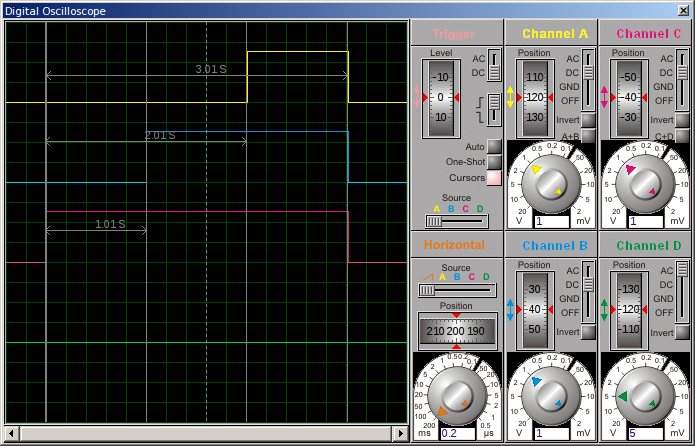
\includegraphics[width=0.45\textwidth]{cap5_scheduler_p_pro1a.png}}
	\subfigure[Atraso: s]{\label{fig:cap5_scheduler_p_pro1b}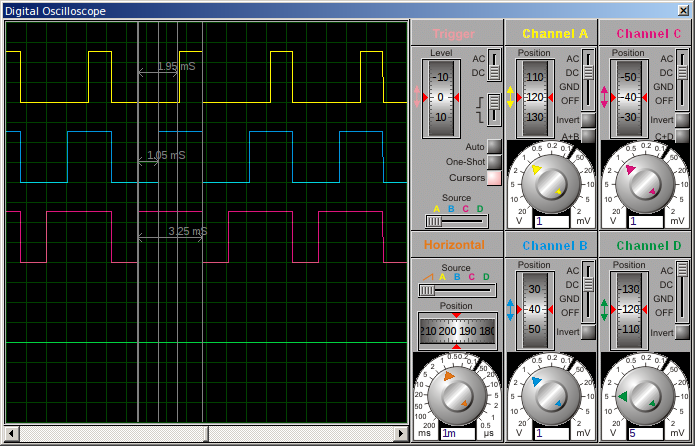
\includegraphics[width=0.45\textwidth]{cap5_scheduler_p_pro1b.png}}
	\label{fig:cap5_scheduler_p_pro1}
\end{figure}

Uma demonstração do circuito em funcionamento pode ser visualizada em \url{https://youtu.be/TBPQiTFyujo}. Para melhor observação do comportamento do sistema foram definidos atrasos de 1 segundo.

\subsection{Experimento 2: Escalonador por Round-Robin}

Diferente do escalonador por prioridades, o escalonamento por \emph{Round-Robin} é realizado por uma interrupção temporal, a qual ocorre apenas quando mais de uma tarefa com a mesma prioridade estejam ativas ao mesmo tempo, podendo estas tarefas serem tanto de tipos diferentes quanto múltiplas ativações de um mesmo tipo. Para fins deste teste, todas as tarefas estão limitadas a apenas uma ativação e são de tipos diferentes, cada qual responsável por um dos LEDs do circuito. O código fonte deste experimento pode ser visualizado no \refalg{cap5_scheduler_rr_program}, junto de seu arquivo de configuração OIL em \refalg{cap5_scheduler_rr_oil}, ambos listados no \refape{capA_validacao}.

\subsubsection{Configuração do Experimento}

Assim como no escalonador por prioridades\refcap{cap5_scheduler_p}, foram utilizadas 5 tarefas, onde uma delas ficou responsável pela inicialização das outras, uma pelo desligamento dos LEDs e as demais pelo acendimento do LED de seu respectivo processo. Diferente do teste anterior, com exceção da tarefa \texttt{task\_init}, nenhuma das outras tarefas encerra sua execução, permanecendo infinitamente ativas, até que o microcontrolador seja desligado.

Como todas as tarefas possuem a mesma prioridade, a ordem de execução se dá exclusivamente pela ordem de ativação das tarefas, conforme especificado pelas linhas 7 à 10 do \refalg{cap5_scheduler_rr_program} do \refape{capA_validacao}. O diagrama de estados presente na \reffig{cap5_scheduler_rr} ilustra a ordem de execução destas tarefas.

\figura{cap5_scheduler_rr}{Diagrama de estados do escalonador por Round-Robin}{7cm}{}

\subsubsection{Resultados}

Assim como no teste anterior, o comportamento do sistema foi exatamente como o especificado pela norma. A cada intervalo de $1_{ms}$, valor adotado pelo OpenAUTOS como o intervalo de escalonamento para Round-Robin, ou seja, o valor do quantum, uma interrupção é gerada pelo temporizador do sistema. Durante esta interrupção, faz-se uma busca pela próxima tarefa de mesma prioridade que se encontra ativa\footnote{No estado \texttt{READY}.}, fazendo com que haja uma troca de contexto em caso afirmativo. Importante ressaltar que esta é a única forma encontrada pela norma de troca de contexto em uma interrupção. Nos demais casos, mesmo que uma tarefa seja ativada durante uma interrupção, ela só será considerada no próximo ponto de escalonamento\footnote{Que se resumem as rotinas: \texttt{Schedule}, \texttt{ActivateTask}, \texttt{TerminateTask}, \texttt{ChainTask}, \texttt{SetEvent}, \texttt{WaitEvent} e \texttt{ReleaseResource}.}.

O resultado da execução deste teste, tanto no modelo físico quanto no virtual, pode ser visualizado na \reffig{cap5_scheduler_rr_osc} e na \reffig{cap5_scheduler_rr_pro}.

\figura{cap5_scheduler_rr_osc}{Escalonador por \emph{Round-Robin} - Osciloscópio}{7cm}{}

\figura{cap5_scheduler_rr_pro}{Escalonador por \emph{Round-Robin} - Proteus}{7cm}{}

Uma demonstração do circuito em funcionamento está disponível em \url{https://youtu.be/QC50OuNeoio}. Para uma melhor visualização do experimento foi aumentado para $1_s$ o tempo de interrupção para chamada do escalonador \emph{Round-Robin}.

\subsection{Experimento 3: Escalonador por Prioridade e Round-Robin}

Este experimento teve como objetivo avaliar o funcionamento do SO em um cenário onde ambos os modelos de escalonamento seriam requisitados. O código para este experimento está disponibilizado no \refalg{cap5_scheduler_prr_program} bem como no arquivo de configuração OIL em \refalg{cap5_scheduler_prr_oil}, ambos listados no \refape{capA_validacao}.

\subsubsection{Configuração do Experimento}

Foram utilizados 5 tipos de tarefas, os quais ficaram organizados da seguinte maneira:

\begin{itemize}
	\item \textbf{\texttt{task\_init}}: tarefa com a menor prioridade, e a única que nunca é encerrada. Ela tem por objetivo manter o programa em ciclo após o encerramento de todas as tarefas de maior prioridade que ela;
	\item \textbf{\texttt{task\_start}}: ativada pela tarefa \textbf{\texttt{task\_init}}, seu papel é o de apagar os LEDS, bem como o de ativar as tarefas que os reacenderão;
	\item \textbf{\texttt{task\_b\textit{n}}}: são as tarefas responsáveis pelo acendimento de seu respectivo LED. Todas possuem a mesma prioridade e também fazem uso a uma chamada na rotina de atraso, para permitir que o tempo de escalonamento do \emph{Round-Robin} execute pelo menos uma vez para cada uma destas tarefas.
\end{itemize}

A \reffig{cap5_scheduler_prr} apresenta um diagrama de estados deste teste, com os seguintes destaques:

\begin{itemize}
	\item Em cinza encontram-se as tarefas que são escalonados pelas rotinas de prioridade;
	\item Em rosa encontram-se as tarefas que possuem mesma prioridade e que são escalonadas por \emph{Round-Robin};
	\item Em preto encontram-se as setas indicando transições que ocorrem exclusivamente por \texttt{TerminateTask};
	\item Em azul encontram-se as setas indicando transições que ocorrem tanto por interrupção quanto por \texttt{TerminateTask};
\end{itemize}

\figura{cap5_scheduler_prr}{Diagrama de estados do escalonador por Prioridade e Round-Robin}{7cm}{}

\subsubsection{Resultados}

O experimento se comportou conforme o esperado onde, em um primeiro momento, o sistema faz a ativação das tarefas através de chamadas a rotina \texttt{ActivateTask}, até então escalonando apenas pela tarefa de maior prioridade ativa na ocasião, que pela lógica do programa acontece na seguinte ordem: \texttt{task\_init}, \texttt{task\_start} e \texttt{task\_b0}.

No momento em que \texttt{task\_b0} entra em execução, apenas tarefas de prioridade idêntica estão ativas no sistema. A partir deste momento, o sistema passa a escalonar as tarefas por \emph{Round-Robin} nos intervalos de quantum definidos pelo SO. O sistema permanece, então, neste modelo de escalonamento até que as tarefas terminem seu tempo de atraso, encerrando, prematuro ao quantum, seu funcionamento através da rotina \texttt{TerminateTask}.

Uma vez encerrada a última das tarefas de ativação de LEDs, a tarefa \texttt{task\_init} volta a ser a tarefa de maior prioridade no sistema, reiniciando o processo.

As ondas dos osciloscópios das figuras \ref{fig:cap5_scheduler_prr_osc} e \ref{fig:cap5_scheduler_prr_pro} ilustram o momento em que as tarefas de acionamento dos LEDs são iniciadas e o tempo no qual elas permanecem processando a rotina de atraso.

\figura{cap5_scheduler_prr_osc}{Escalonador por prioridade e \emph{Round-Robin} - Osciloscópio}{7cm}{}

\figura{cap5_scheduler_prr_pro}{Escalonador por prioridade e \emph{Round-Robin} - Proteus}{7cm}{}

Um vídeo demonstrativo do funcionamento deste circuito encontra-se disponível em \url{https://youtu.be/LSDL_LMfO3o}, também utilizando atrasos de $1_s$ para permitir uma melhor observação do fluxo de funcionamento.

\subsection{Experimento 4: Alocação de Recursos}

Assim como no modelo de prioridade com \emph{Round-Robin}, este experimento utilizou um cenário bem semelhante, porém, com o uso da alocação de recursos e prioridade-teto para que um processo de baixa prioridade pudesse ativar tarefas de maior prioridade sem ser escalonado imediatamente. O código fonte deste experimento pode ser encontrado em \refalg{cap5_scheduler_res_program}, junto de seu arquivo de configuração OIL em \refalg{cap5_scheduler_res_oil}, ambos listados no \refape{capA_validacao}.

\subsubsection{Configuração do Experimento}

Diferente dos outros experimentos, foram utilizadas apenas 4 tarefas, onde:

\begin{itemize}
	\item \textbf{\texttt{task\_init}}: além de fazer a inicialização das portas utilizadas, também é responsável por apagar os LEDs e ativar as tarefas que os reacenderão. Por possuir uma prioridade inferior a das tarefas dos LEDs, \textbf{\texttt{task\_init}} primeiro aloca um recurso de maior prioridade que as tarefas antes de ativá-las. Por fim, esta tarefa é escalonada assim que tem sua prioridade restaurada ao normal, logo após a chamada a rotina \emph{ReleaseResource}. este processo de alocação do recurso pode ser visualizado no diagrama de sequência na \reffig{cap5_scheduler_res};
	\item \textbf{\texttt{task\_b\textit{n}}}: tarefas que realizam o acendimento dos LEDS.
\end{itemize}

\figura{cap5_scheduler_res}{Diagrama de sequencia da alocação de recurso e prioridade-teto}{7cm}{}

\subsubsection{Resultados}

Após a alocação do recurso, a tarefa \texttt{task\_init} passou a ter uma prioridade superior a das tarefas que estaria ativando, permitindo que ativasse todas as tarefas \texttt{task\_b\textit{n}} sem que ela própria fosse escalonada.

A partir do momento no qual o recurso alocado por \texttt{task\_init} é liberado, esta tem sua prioridade reduzida para seu valor original, o qual é inferior ao das demais tarefas que se encontram aptos para execução. Sendo assim, o SO passa a executar as tarefas de maior prioridade, que por possuírem valores idênticos de prioridade, são escalonados por \emph{Round-Robin} até que sua execução encerre com a chamada a rotina \emph{TerminateTask}, reiniciando o clico em \texttt{task\_init}.

Caso \texttt{task\_init} tentasse ativar as demais tarefas sem antes ter feito a alocação do recurso, o SO teria interrompido seu processamento ao retornar da rotina \emph{ActivateTask}, executando cada tarefa até seu encerramento em \emph{TerminateTask}, sem nunca escalonalas por \emph{Round-Robin}.

Os resultados da execução deste experimento podem ser vistos nos gráficos da \reffig{cap5_scheduler_res_osc} e \reffig{cap5_scheduler_res_pro}.

\figura{cap5_scheduler_res_osc}{Alocação de recurso e prioridade-teto - Osciloscópio}{7cm}{}

\figura{cap5_scheduler_res_pro}{Alocação de recurso e prioridade-teto - Proteus}{7cm}{}

Um vídeo demonstrativo do funcionamento deste circuito encontra-se disponível em \url{https://youtu.be/XbD-STWvOCU}, também utilizando atrasos de $1_s$ para permitir uma melhor observação do fluxo de funcionamento.

\section{Dificuldades}

Diversas foram as dificuldades encontradas para o desenvolvimento deste projeto. Na sequência serão descritas algumas delas.

\subsection{Geração de Instruções Defeituosas pelo Compilador XC8}

Por razões desconhecidas, a instrução \texttt{movff}, em Assembly, muitas vezes não realizava nenhuma ação, principalmente quando utilizada com alguns registradores especiais, como os \texttt{TOSU}, \texttt{TOSH} e \texttt{TOSL}, utilizados para manipulação da pilha dos microcontroladores da linha PIC18F, bem como os registradores \texttt{TMR0} e \texttt{TMR1}, utilizados para calcular o tempo de estouro de seus respectivos temporizadores\footnote{Escrever um valor literal nestes registradores sempre resulta em um código operante, pois o compilador passa a utilizar o comando \texttt{movlf} ao invés de \texttt{movff}.}.

Esta instrução é automaticamente utilizada pelo compilador XC8 e, na maioria dos casos, funciona corretamente. Infelizmente, para estes casos onde ela não funcionou, foi necessário que uma parte de código Assembly fosse escrito manualmente para contornar o seu uso.

\subsection{Seleção de Bancos de Memória}

Devido a grande quantidade de memória alocada estaticamente pelo OpenAUTOS e tarefas definidas pelo usuário, um dos inconvenientes que passou a ser notado foram as indicações de bancos de memória cheios.

Idealmente, ele deveria ser capaz de declarar estas variáveis que excederiam o limite de um banco de memória em um outro banco automaticamente. Porém, o compilador não estava realizando esta operação, que teve que ser realizada manualmente a partir de instruções Assembly.

Um outro inconveniente que passou a ser observado foi a má distribuição dos espaços presentes nos bancos de memória do microcontrolador, o que pode ser notado no arquivo de extensão \emph{lst} gerado durante a compilação da imagem do hardware, onde há diversas segmentações de memória e a maioria dos bancos apresentam um espaço considerável ainda.

Por este projeto utilizar apenas a versão gratuita do compilador, e também por ter suas compilações apenas em modo de \emph{Debug}, acredita-se que diversas otimizações ainda possam ser alcançadas neste quesito.

\subsection{Ferramentas de Depuração}

Embora de grande ajuda na depuração de \emph{bugs}, algumas vezes as ferramentas MPLAB e Proteus não conseguem acompanhar perfeitamente os formatos de imagem para depuração suportados pelo compilador XC8, que são o \emph{elf} e \emph{cof}, o que acaba forçando o desenvolvedor a buscar meios alternativos de buscar informações em uma determinada área de código, geralmente resultando no uso de LEDs para indicar estados do sistema.

\subsection{Abrangência da Norma}

Mesmo com a alta disponibilidade de informações sobre projetos e artigos que atuam nas normas do OSEK/VDX e AUTOSAR, pouquíssimos são aqueles se aprofundam nos temas. Isto implica que a maior parte das informações devem ser extraídas diretamente das normas, o que passa a ser um processo trabalhoso devido a extensão e complexidade das mesmas.

É, também, difícil de acompanhar e levantar todos os detalhes referentes a cada módulo proposto, já que as normas costumam separar informações entre elas que complementam estes sistemas.


\chapter{Considerações Finais}

O desenvolvimento de um sistema operacional embarcado é uma tarefa extensa, desafiadora e complexa, tendo em vista a quantidade funcionalidades que este deve oferecer, bem como a estabilidade, desempenho, portabilidade, dentre vários outros aspectos possíveis.

Desenvolver um SOE que visa atender a um conjunto de normas como as do OSEK/VDX e AUTOSAR apresentou-se um desafio ainda maior do que o que era originalmente esperado, tamanha a complexidade do sistema proposto por elas.

Embora o trabalho tenha apresentado sucesso no desenvolvimento parcial de um SOE baseado nestas normas, existem ainda diversos módulos e funcionalidades que precisam serem implementadas para que o SOE se adeque totalmente as normas.

Este trabalho tem sua importância marcada como o inicio do SOE OpenAUTOS que, no momento, oferece uma estrutura preparada para o desenvolvimento em múltiplas plataformas de micro-controladores, um compilador para a linguagem OIL, sistemas para o gerenciamento de tarefas, trocas de contexto e alocação de recursos, bem como uma base de código para a implementação das demais funcionalidades.

Embora todas estas funcionalidades tenham sido testadas e validadas conforme especifica a norma, há ainda bastante espaço para melhorias, pois muitas das funções e estruturas de dados utilizadas foram implementadas sem revisões de otimização ou um planejamento de longo prazo, com o intuito de deixar o OpenAUTOS em um ponto usável o mais cedo possível, para que a partir dali ele evoluísse para um sistema mais complexo.

Espera-se que o OpenAUTOS continue a evoluir, mesmo com a conclusão deste trabalho, e que, eventualmente, ele venha a se tornar uma referência no mercado de sistemas embarcados automobilísticos, tanto como uma ferramenta de ensino como em usabilidade. Para isso, seu código está disponível no repositório online GitHub, sobre o endereço \url{https://github.com/brunocanella/OpenAUTOS}.

\section{Propostas para Trabalhos Futuros}

Neste seção são listadas algumas propostas como trabalhos futuros que visam estender e melhorar o SOE OpenAUTOS:

\begin{enumerate}
	\item Implementar os módulos restantes para a conclusão do SO, conforme a norma do OSEK/VDX;
	\item Implementar as funcionalidades de SO acrescentada pelas normas do AUTOSAR;
	\item Realizar \emph{benchmarks} comparativos com outras soluções em SOE disponiveis;
	\item Fazer o porte do SOE OpenAUTOS para outros microcontroladores;
	\item Otimizar o espaço de memória utilizado pelo SO, principalmente quanto ao aproveitamento dos espaços nos bancos de memória dos microcontroladores PIC18F;
	\item Iniciar o desenvolvimento dos modulos complementares ao SOE, como a \criarSigla{Run-Time Environment}{RTE} do AUTOSAR, ou ainda as normas de comunicação do OSEK-COM;
	\item Desenvolver um projeto veícular que utilize como SOE o OpenAUTOS.
\end{enumerate}


%--------------------------------------------------------
%Referências

\bibliographystyle{ufscThesis/ufsc-alf}
\bibliography{referencias}

%-------------------------\textsl{}-------------------------------
% Elementos pós-textuais
\apendice
\chapter{Algoritmos dos Testes de Validação do OpenAUTOS} \label{ape:capA_validacao}

\begin{algoritmo}{cap5_scheduler_p_program}{Algoritmo do escalonador por prioridade}{c}
TASK( task_init ) {
	TRISB = 0x00; // Output Lower Bits
	LATB = 0x00;
	
	ChainTask( task_start );
}
#define _XTAL_FREQ 64000000
TASK( task_rb0 ) {
	LATBbits.LATB0 = 1;
	__delay_ms(1);
	ChainTask(task_start);	
}
TASK( task_rb1 ) {
	LATBbits.LATB1 = 1;
	__delay_ms(1);
	TerminateTask();
}
TASK( task_rb2 ) {
	LATBbits.LATB2 = 1;
	__delay_ms(1);
	TerminateTask();
}
TASK( task_start ) {
	LATB = 0;
	__delay_ms(1);
	ActivateTask( task_rb0 );
	ActivateTask( task_rb1 );
	ActivateTask( task_rb2 );
	TerminateTask();
}
\end{algoritmo}

\begin{algoritmo}{cap5_scheduler_p_oil}{Configuração OIL do escalonador por prioridade}{c}
OIL_VERSION = "2.5" "DESC_OIL_VERSION";

CPU PIC18F25K80 {
	OS OpenAUTOS {
		STATUS = EXTENDED;
		STARTUPHOOK = TRUE;
		ERRORHOOK = TRUE;
		SHUTDOWNHOOK = FALSE;
		PRETASKHOOK = FALSE;
		POSTTASKHOOK = FALSE;
		USEGETSERVICEID = TRUE;
		USEPARAMETERACCESS = TRUE;
		USERESSCHEDULER = TRUE;
	} "DESC_OS";
	
	TASK task_rb0 {
		PRIORITY = 1;
		SCHEDULE = FULL;
		ACTIVATION = 1;
		AUTOSTART = FALSE;
	};
	TASK task_rb1 {
		PRIORITY = 2;
		SCHEDULE = FULL;
		ACTIVATION = 1;
		AUTOSTART = FALSE;
	};
	TASK task_rb2 {
		PRIORITY = 3;
		SCHEDULE = FULL;
		ACTIVATION = 1;
		AUTOSTART = FALSE;
	};
	TASK task_start {
		PRIORITY = 5;
		SCHEDULE = FULL;
		ACTIVATION = 1;
		AUTOSTART = FALSE;
	};
	TASK task_init {
		PRIORITY = 254;
		SCHEDULE = FULL;
		ACTIVATION = 1;
		AUTOSTART = TRUE {
			APPMODE = AppMode0;
		};
	};	
};
\end{algoritmo}

\begin{algoritmo}{cap5_scheduler_rr_program}{Algoritmo do escalonador por \emph{Round-Robin}}{c}
TASK( task_init ) {
	TRISB = 0x00; // Output Lower Bits
	LATB = 0x00;
	
	ActivateTask( task_rb0 );
	ActivateTask( task_rb1 );
	ActivateTask( task_rb2 );
	ActivateTask( task_off );
	TerminateTask();
}

TASK( task_rb0 ) {
	while( TRUE ) {
		LATBbits.LATB0 = 1;
	}
}

TASK( task_rb1 ) {
	while( TRUE ) {
		LATBbits.LATB1 = 1;
	}
}

TASK( task_rb2 ) {
	while( TRUE ) {
		LATBbits.LATB2 = 1;
	}
}

TASK( task_off ) {	
	while( TRUE ) {
		LATB = 0;
	}
}
\end{algoritmo}

\begin{algoritmo}{cap5_scheduler_rr_oil}{Configuração OIL do escalonador por \emph{Round-Robin}}{c}
OIL_VERSION = "2.5" "DESC_OIL_VERSION";

CPU PIC18F25K80 {
	OS OpenAUTOS {
		STATUS = EXTENDED;
		STARTUPHOOK = TRUE;
		ERRORHOOK = TRUE;
		SHUTDOWNHOOK = FALSE;
		PRETASKHOOK = FALSE;
		POSTTASKHOOK = FALSE;
		USEGETSERVICEID = TRUE;
		USEPARAMETERACCESS = TRUE;
		USERESSCHEDULER = TRUE;
	} "DESC_OS";
	
	TASK task_rb0 {
		PRIORITY = 1;
		SCHEDULE = FULL;
		ACTIVATION = 1;
		AUTOSTART = FALSE;
	};
	TASK task_rb1 {
		PRIORITY = 1;
		SCHEDULE = FULL;
		ACTIVATION = 1;
		AUTOSTART = FALSE;
	};
	TASK task_rb2 {
		PRIORITY = 1;
		SCHEDULE = FULL;
		ACTIVATION = 1;
		AUTOSTART = FALSE;
	};
	TASK task_off {
		PRIORITY = 1;
		SCHEDULE = FULL;
		ACTIVATION = 1;
		AUTOSTART = FALSE;
	};
	TASK task_init {
		PRIORITY = 254;
		SCHEDULE = FULL;
		ACTIVATION = 1;
		AUTOSTART = TRUE {
			APPMODE = AppMode0;
		};
	};	
};
\end{algoritmo}

\begin{algoritmo}{cap5_scheduler_prr_program}{Algoritmo do escalonador por prioridade e \emph{Round-Robin}}{c}
#include <stdint.h>

#define _XTAL_FREQ 64000000

void delay_s( uint8_t s ) {
	while( s > 0 ) {
		s--;
		for( uint8_t i = 0; i < 100; i++ ) {
			__delay_ms(10);
		}
	}
}

TASK( task_init ) {
	TRISB = 0x00; // Output Lower Bits
	LATB = 0x00;
	
	while( TRUE ) {
		ActivateTask( task_start );		
	}
}

TASK( task_start ) {		
	ActivateTask( task_rb0 );
	ActivateTask( task_rb1 );
	ActivateTask( task_rb2 );	
	LATB = 0;
	TerminateTask();
}

TASK( task_rb0 ) {
	LATBbits.LATB0 = 1;
	delay_s(2);
	TerminateTask();
}

TASK( task_rb1 ) {
	LATBbits.LATB1 = 1;
	delay_s(2);
	TerminateTask();
}

TASK( task_rb2 ) {
	LATBbits.LATB2 = 1;
	delay_s(2);
	TerminateTask();
}
\end{algoritmo}

\begin{algoritmo}{cap5_scheduler_prr_oil}{Configuração OIL do escalonador por prioridade e \emph{Round-Robin}}{c}
OIL_VERSION = "2.5" "DESC_OIL_VERSION";

CPU PIC18F25K80 {
	OS OpenAUTOS {
		STATUS = EXTENDED;
		STARTUPHOOK = TRUE;
		ERRORHOOK = TRUE;
		SHUTDOWNHOOK = FALSE;
		PRETASKHOOK = FALSE;
		POSTTASKHOOK = FALSE;
		USEGETSERVICEID = TRUE;
		USEPARAMETERACCESS = TRUE;
		USERESSCHEDULER = TRUE;
	} "DESC_OS";
	
	TASK task_rb0 {
		PRIORITY = 2;
		SCHEDULE = FULL;
		ACTIVATION = 1;
		AUTOSTART = FALSE;
	};
	TASK task_rb1 {
		PRIORITY = 2;
		SCHEDULE = FULL;
		ACTIVATION = 1;
		AUTOSTART = FALSE;
	};
	TASK task_rb2 {
		PRIORITY = 2;
		SCHEDULE = FULL;
		ACTIVATION = 1;
		AUTOSTART = FALSE;
	};
	TASK task_start {
		PRIORITY = 3;
		SCHEDULE = FULL;
		ACTIVATION = 1;
		AUTOSTART = FALSE;
	};
	TASK task_init {
		PRIORITY = 1;
		SCHEDULE = FULL;
		ACTIVATION = 1;
		AUTOSTART = TRUE {
			APPMODE = AppMode0;
		};
	};	
};
\end{algoritmo}

\begin{algoritmo}{cap5_scheduler_res_program}{Algoritmo da alocação de recurso e prioridade-teto}{c}
#include <stdint.h>

#define _XTAL_FREQ 64000000

void delay_s( uint8_t s ) {
	while( s > 0 ) {
		s--;
		for( uint8_t i = 0; i < 100; i++ ) {
			__delay_ms(10);
		}
	}
}

TASK( task_init ) {
	TRISB = 0x00; // Output Lower Bits
	LATB = 0x00;
	
	while( TRUE ) {
		GetResource( res_a );
		ActivateTask( task_rb0 );
		ActivateTask( task_rb1 );
		ActivateTask( task_rb2 );
		LATB = 0;
		delay_s(1);
		ReleaseResource( res_a );
	}
}

TASK( task_rb0 ) {
	LATBbits.LATB0 = 1;
	delay_s(1);
	TerminateTask();
}

TASK( task_rb1 ) {
	LATBbits.LATB1 = 1;
	delay_s(1);
	TerminateTask();
}

TASK( task_rb2 ) {
	LATBbits.LATB2 = 1;
	delay_s(1);
	TerminateTask();
}
\end{algoritmo}

\begin{algoritmo}{cap5_scheduler_res_oil}{Configuração OIL da alocação de recurso e prioridade-teto}{c}
OIL_VERSION = "2.5" "DESC_OIL_VERSION";

CPU PIC18F25K80 {
	OS OpenAUTOS {
		STATUS = EXTENDED;
		STARTUPHOOK = TRUE;
		ERRORHOOK = TRUE;
		SHUTDOWNHOOK = FALSE;
		PRETASKHOOK = FALSE;
		POSTTASKHOOK = FALSE;
		USEGETSERVICEID = TRUE;
		USEPARAMETERACCESS = TRUE;
		USERESSCHEDULER = TRUE;
	} "DESC_OS";
	
	TASK task_rb0 {
		PRIORITY = 2;
		SCHEDULE = FULL;
		ACTIVATION = 1;
		AUTOSTART = FALSE;
	};
	TASK task_rb1 {
		PRIORITY = 2;
		SCHEDULE = FULL;
		ACTIVATION = 1;
		AUTOSTART = FALSE;
	};
	TASK task_rb2 {
		PRIORITY = 2;
		SCHEDULE = FULL;
		ACTIVATION = 1;
		AUTOSTART = FALSE;
	};
	
	TASK task_init {
		PRIORITY = 1;
		SCHEDULE = FULL;
		ACTIVATION = 1;
		AUTOSTART = TRUE {
			APPMODE = AppMode0;
		};
		RESOURCE = res_a;
	};
	RESOURCE res_a {
		RESOURCEPROPERTY = STANDARD;
	};
};
\end{algoritmo}
%\apendice
%\chapter{Exemplificando um Apêndice}
%Texto do Apêndice aqui. 

\anexo
\chapter{OpenAUTOS API: OSEK/VDX}

\begin{algoritmo}{ane_openautos_api_osek_hook}{Interfaces do OSEK/VDX - Rotinas de Hooks}{c}
/**
* @brief This hook routine is called by the operating system at the end of a system service which returns StatusType not equal E_OK. It is called before returning to the task level.
* @brief This hook routine is called when an alarm expires and an error is detected during task activation or event setting.
* @brief The ErrorHook is not called, if a system service called from ErrorHook does not return E_OK as status value. Any error by calling of system services from the ErrorHook can only be detected by evaluating the status value.
*
* @remark See chapter 11.1 for general description of hook routines.
*
* @param[in] Error The Error occurred.
*/
void ErrorHook( StatusType Error );

/**
* This hook routine is called by the operating system before executing a new task, but after the transition of the task to the running state (to allow evaluation of the TaskID by GetTaskID).
* 
* @remark See chapter 11.1 for general description of hook routines.
*/
void PreTaskHook( void );

/**
* This hook routine is called by the operating system after executing the current task, but before leaving the task's running state (to allow evaluation of the TaskID by GetTaskID).
*
* @remark See chapter 11.1 for general description of hook routines.
*/
void PostTaskHook( void );

/**
* This hook routine is called by the operating system at the end of the operating system initialisation and before the scheduler is running. At this time the application can initialise device drivers etc.
*
* @remark See chapter 11.1 for general description of hook routines.
*/
void StartupHook( void );

/**
* This hook routine is called by the operating system when the OS service ShutdownOS has been called. This routine is called during the operating system shut down.
*
* @remark ShutdownHook is a hook routine for user defined shutdown functionality, see chapter 11.4.
*
* @param[in] Error Error occurred
*/
void ShutdownHook( StatusType Error );
\end{algoritmo}

\begin{algoritmo}{ane_openautos_api_osek_int}{Interfaces do OSEK/VDX - Rotinas de Interrupção}{c}
/**
* This service restores the state saved by DisableAllInterrupts.
* @remark The service may be called from an ISR category 1 and category 2 and from the task level, but not from hook routines.
* @remark This service is a counterpart of DisableAllInterrupts service, which has to be called before, and its aim is the completion of the critical section of code. No API service calls are allowed within this critical section.
* @remark The implementation should adapt this service to the target hardware providing a minimum overhead. Usually, this service enables recognition of interrupts by the central processing unit.
*/
void EnableAllInterrupts( void );

/**
* This service disables all interrupts for which the hardware supports disabling. The state before is saved for the EnableAllInterrupts call.
* 
* @remark The service may be called from an ISR category 1 and category 2 and from the task level, but not from hook routines.
* @remark This service is intended to start a critical section of the code. 
* @remark This section shall be finished by calling the EnableAllInterrupts service. No API service calls are allowed within this critical section.
* @remark The implementation should adapt this service to the target hardware providing a minimum overhead. Usually, this service disables recognition of interrupts by the central processing unit.
* @remark Note that this service does not support nesting. If nesting is needed for critical sections e.g: for libraries SuspendOSInterrupts/ResumeOSInterrupts or SuspendAllInterrupt/ResumeAllInterrupts should be used.
*/
void DisableAllInterrupts( void );


/**
* This service restores the recognition status of all interrupts saved by the SuspendAllInterrupts service.
* 
* @remark The service may be called from an ISR category 1 and category 2, from alarm-callbacks and from the task level, but not from all hook routines.
* @remark This service is the counterpart of SuspendAllInterrupts service, which has to have been called before, and its aim is the completion of the critical section of code. No API service calls beside SuspendAllInterrupts/ResumeAllInterrupts pairs and SuspendOSInterrupts/ResumeOSInterrupts pairs are allowed within this critical section.
* @remark The implementation should adapt this service to the target hardware providing a minimum overhead. 
* @remark SuspendAllInterrupts/ResumeAllInterrupts can be nested. In case of nesting pairs of the calls SuspendAllInterrupts and ResumeAllInterrupts the interrupt recognition status saved by the first call of SuspendAllInterrupts is restored by the last call of the ResumeAllInterrupts service.
*/
void ResumeAllInterrupts( void );

/**
* This service saves the recognition status of all interrupts and disables all interrupts for which the hardware supports disabling.
* @remark The service may be called from an ISR category 1 and category 2, from alarm-callbacks and from the task level, but not from all hook routines.
* @remark This service is intended to protect a critical section of code from interruptions of any kind. This section shall be finished by calling the ResumeAllInterrupts service. No API service calls beside SuspendAllInterrupts/ResumeAllInterrupts pairs and SuspendOSInterrupts/ResumeOSInterrupts pairs are allowed within this critical section.
* @remark The implementation should adapt this service to the target hardware providing a minimum overhead.
*/
void SuspendAllInterrupts( void );

/**
* This service restores the recognition status of interrupts saved by the SuspendOSInterrupts service.
* 
* @remark The service may be called from an ISR category 1 and category 2 and from the task level, but not from hook routines.
* @remark This service is the counterpart of SuspendOSInterrupts service, which has to have been called before, and its aim is the completion of the critical section of code. No API service calls beside SuspendAllInterrupts/ResumeAllInterrupts pairs and SuspendOSInterrupts/ResumeOSInterrupts pairs are allowed within this critical section.
* @remark The implementation should adapt this service to the target hardware providing a minimum overhead.
* @remark SuspendOSInterrupts/ResumeOSInterrupts can be nested. In case of nesting pairs of the calls SuspendOSInterrupts and ResumeOSInterrupts the interrupt recognition status saved by the first call of SuspendOSInterrupts is restored by the last call of the ResumeOSInterrupts service.
*/
void ResumeOSInterrupts( void );

/**
* This service saves the recognition status of interrupts of category 2 and disables the recognition of these interrupts.
* @remark The service may be called from an ISR and from the task level, but not from hook routines.
* @remark This service is intended to protect a critical section of code. This section shall be finished by calling the ResumeOSInterrupts service. No API service calls beside SuspendAllInterrupts/ResumeAllInterrupts pairs and SuspendOSInterrupts/ResumeOSInterrupts pairs are allowed within this critical section.
* @remark The implementation should adapt this service to the target hardware providing a minimum overhead.
* @remark It is intended only to disable interrupts of category 2. However, if this is not possible in an efficient way more interrupts may be disabled.
*/
void SuspendOSInterrupts( void );
\end{algoritmo}

\begin{algoritmo}{ane_openautos_api_osek_os}{Interfaces do OSEK/VDX - Rotinas de SO}{c}
/**
* This service returns the current application mode. It may be used to write mode dependent code.
* 
* @remark See chapter 5 for a general description of application modes.
* @remark Allowed for task, ISR and all hook routines.
*
* @return The current application mode.
* 
* @remark [Conformance] BCC1, BCC2, ECC1, ECC2
*/
AppModeType GetActiveApplicationMode( void );

/**
* The user can call this system service to start the operating system in a specific mode, see chapter 5, Application modes.
*
* @remark Only allowed outside of the operating system, therefore implementation specific restrictions may apply. See also chapter 11.3, System start-up, especially with respect to systems where OSEK and OSEKtime coexist. This call does not need to return.
*
* @param[in] Mode The application mode to start the OS.
* 
* @remark [Conformance] BCC1, BCC2, ECC1, ECC2
*/
void StartOS( AppModeType Mode );

/**
* @brief The user can call this system service to abort the overall system (e.g. emergency off). The operating system also calls this function internally, if it has reached an undefined internal state and is no longer ready to run.
* @brief If a ShutdownHook is configured the hook routine ShutdownHook is always called (with <Error> as argument) before shutting down the operating system. If ShutdownHook returns, further behaviour of ShutdownOS is implementation specific.
* @brief In case of a system where OSEK OS and OSEKtime OS coexist, ShutdownHook has to return.
* @brief <Error> needs to be a valid error code supported by OSEK OS. In case of a system where OSEK OS and OSEKtime OS coexist, <Error> might also be a value accepted by OSEKtime OS. In this case, if enabled by an OSEKtime configuration parameter, OSEKtime OS will be shut down after OSEK OS shutdown.
*
* @remark After this service the operating system is shut down.
* @remark Allowed at task level, ISR level, in ErrorHook and StartupHook, and also called internally by the operating system.
* @remark If the operating system calls ShutdownOS it never uses E_OK as the passed parameter value.
*
* @param[in]  Error  The error
*/
void ShutdownOS( StatusType Error );
\end{algoritmo}
	
\begin{algoritmo}{ane_openautos_api_osek_res}{Interfaces do OSEK/VDX - Rotinas de Recursos}{c}
/**
* DeclareResource serves as an external declaration of a resource. The function and use of this service are similar to that of the external declaration of variables.
*
* @param[in] ResourceIdentifier Resource identifier (Duh).
*/
#define DeclareResource( ResourceIdentifier ) extern ResourceType ##ResourceIdentifier;

/**
* This call serves to enter critical sections in the code that are assigned to the resource referenced by ResID. A critical section shall always be left using ReleaseResource.
*
* @remark The OSEK priority ceiling protocol for resource management is described in chapter 8.5.
* @remark Nested resource occupation is only allowed if the inner critical sections are completely executed within the surrounding critical section (strictly stacked, see chapter 8.2, Restrictions when using resources). Nested occupation of one and the same resource is also forbidden!
* @remark It is recommended that corresponding calls to GetResource and ReleaseResource appear within the same function.
* @remark It is not allowed to use services which are points of rescheduling for non preemptable tasks (TerminateTask, ChainTask, Schedule and WaitEvent, see chapter 4.6.2) in critical sections. Additionally, critical sections are to be left before completion of an interrupt service routine.
* @remark Generally speaking, critical sections should be short.
* @remark The service may be called from an ISR and from task level (see Figure 12-1).
*
* @param[in] ResID Reference to resource
*
* @return [Standard] No error, E_OK.
* @return [Extended] Resource <ResID> is invalid, E_OS_ID.
* @return [Extended] Attempt to get a resource which is already occupied by any task or ISR, or the statically assigned priority of the calling task or interrupt routine is higher than the calculated ceiling priority, E_OS_ACCESS
*/
StatusType GetResource( ResourceType ResID );

/**
* ReleaseResource is the counterpart of GetResource and serves to leave critical sections in the code that are assigned to the resource referenced by ResID.
*
* @param[in] ResID Reference to resource.
*
* @remark For information on nesting conditions, see particularities of GetResource.
* @remark The service may be called from an ISR and from task level (see Figure 12-1).
* 
* @return [Standard] No error, E_OK.
* @return [Extended] Resource <ResID> is invalid, E_OS_ID.
* @return Attempt to release a resource which is not occupied by any task or ISR, or another resource shall be released before, E_OS_NOFUNC.
* @return Attempt to release a resource which has a lower ceiling priority than the statically assigned priority of the calling task or interrupt routine, E_OS_ACCESS.
*/
StatusType ReleaseResource( ResourceType ResID );
\end{algoritmo}
	
\begin{algoritmo}{ane_openautos_api_osek_task}{Interfaces do OSEK/VDX - Rotinas de Escalonamento}{c}
/**
* DeclareTask serves as an external declaration of a task. The
* function and use of this service are similar to that of the external
* declaration of variables.
*/
#define DeclareTask( TaskName, TaskID ) const TaskType TaskType_##TaskName = (TaskID)

#define TASK( TaskName ) void TASK_FUNC_##TaskName(void)

////////////////////////////////////////////////////////////////////////////////
//  System Services
////////////////////////////////////////////////////////////////////////////////

/**
* The task TaskID is transferred from the suspended state into the ready state. The operating system ensures that the task code is being executed from the first statement.
*
* @remark When an extended task is transferred from suspended state into ready state all its events are cleared.
*
* @remark The service may be called from interrupt level and from task level (see Figure 12-1). Rescheduling after the call to ActivateTask depends on the place it is called from (ISR, non preemptable task, preemptable task).
*
* If E_OS_LIMIT is returned the activation is ignored.
*
* @param TaskID[in] Task reference
* 
* @return [Standard] No error, E_OK.
* @return [Extended] Too many task activations of TaskID, E_OS_LIMIT
* @return [Extended] Task TaskID is invalid, E_OS_ID
* 
* @remark [Conformance] BCC1, BCC2, ECC1, ECC2
*/
StatusType ActivateTask( TaskType TaskID );

/**
* This service causes the termination of the calling task. The calling task is transferred from the running state into the suspended state.
*
* @remark An internal resource assigned to the calling task is automatically released. Other resources occupied by the task shall have been released before the call to TerminateTask. If a resource is still occupied in standard status the behaviour is undefined.
* @remark If the call was successful, TerminateTask does not return to the call level and the status can not be evaluated. If the version with extended status is used, the service returns in case of error, and provides a status which can be evaluated in the application. If the service TerminateTask is called successfully, it enforces a rescheduling.
* @remark Ending a task function without call to TerminateTask or ChainTask is strictly forbidden and may leave the system in an undefined state.
*
* @return Task still occupies resources, E_OS_RESOURCE
* @return Call at interrupt level, E_OS_CALLEVEL
*/
StatusType TerminateTask( void );

/**
* This service causes the termination of the calling task. After termination of the calling task a succeeding task <TaskID> is activated. Using this service, it ensures that the succeeding task starts to run at the earliest after the calling task has been terminated.
*
* @remark If the succeeding task is identical with the current task, this does not result in multiple requests. The task is not transferred to the suspended state, but will immediately become ready again.
* @remark An internal resource assigned to the calling task is automatically released, even if the succeeding task is identical with the current task. Other resources occupied by the calling shall have been released before ChainTask is called. If a resource is still occupied in standard status the behaviour is undefined.
* @remark If called successfully, ChainTask does not return to the call level and the status can not be evaluated.
* @remark In case of error the service returns to the calling task and provides a status which can then be evaluated in the application.
* @remark If the service ChainTask is called successfully, this enforces a rescheduling.
* @remark Ending a task function without call to TerminateTask or ChainTask is strictly forbidden and may leave the system in an undefined state.
* @remark If E_OS_LIMIT is returned the activation is ignored. When an extended task is transferred from suspended state into ready state all its events are cleared.
*
* @param TaskID[in] Reference to the sequential succeeding task to be activated.
*
* @return [Standard] No return to call level.
* @return [Standard] Too many task activations of <TaskID>, E_OS_LIMIT.
* @return [Extended] Task <TaskID> is invalid, E_OS_ID.
* @return [Extended] Calling task still occupies resources, E_OS_RESOURCE.
* @return [Extended] Call at interrupt level, E_OS_CALLEVEL.
*/
StatusType ChainTask( TaskType TaskID );

/**
* GetTaskID returns the information about the TaskID of the task which is currently running.
* 
* @remark Allowed on task level, ISR level and in several hook routines (see Figure 12-1).
* @remark This service is intended to be used by library functions and hook routines.
* @remark If <TaskID> can’t be evaluated (no task currently running), the service returns INVALID_TASK as TaskType.
*
* @param TaskID[out] Reference to the task which is currently running.
*
* @return [Standard] No error, E_OK
* @return [Extended] No error, E_OK
*/
StatusType GetTaskID( TaskRefType TaskID );

/**
* Returns the state of a task (running, ready, waiting, suspended) at the time 
* of calling GetTaskState.
*
* @remark The service may be called from interrupt service routines, task level, and some hook routines (see Figure 12-1).
* @remark When a call is made from a task in a full preemptive system, the result may already be incorrect at the time of evaluation.
* @remark When the service is called for a task, which is activated more than once, the state is set to running if any instance of the task is running.
*
* @param TaskID[in] Task reference
* @param State[out] Reference to the state of the task TaskID
*
* @return [Standard] No error, E_OK
* @return [Extended] Task TaskID is invalid, E_OS_ID
*/
StatusType GetTaskState( TaskType TaskID, TaskStateRefType State );

/**
* If a higher-priority task is ready, the internal resource of the task is released, the current task is put into the ready state, its context is saved and the higher-priority task is executed. Otherwise the calling task is continued.
*
* @remark Rescheduling only takes place if the task an internal resource is assigned to the calling task during system generation. For these tasks, Schedule enables a processor assignment to other tasks with lower or equal priority than the ceiling priority of the internal resource and higher priority than the priority of the calling task in application-specific locations. When returning from Schedule, the internal resource has been taken again. This service has no influence on tasks with no internal resource assigned (preemptable tasks).
*
* @return [Standard] No error, E_OK.
* @return [Extended] Call at interrupt level, E_OS_CALLEVEL
* @return [Extended] Calling task occupies resources, E_OS_RESOURCE
*/
StatusType Schedule( void );
\end{algoritmo}

\chapter{OpenAUTOS API: Rotinas de Uso Interno do SO}

\begin{algoritmo}{ane_openautos_api_os_resources}{Interfaces do OpenAUTOS - Rotinas de Recursos}{c}
/**Type for the Resource Id*/
typedef uint8_t ResourceType;
/**Type for the Resource ceiling Priority*/
typedef uint8_t ResourceDataPriorityType;

/**
* @brief The structure that stores data about the resource. Also serves as a linked list node
* 
* @remark Due to an odd bug with the xc8 1.37 compiler, where he does not allow it to declare an extern const
* as the size of an array (altough it works sometimes), I changed the model to use "movable" nodes with linked lists.
* 
* Basically, every Task and ISR has a variable which is used as the start of its own linked list. There is also a
* global variable (g_resources) which is the main linked list for resources.
* 
* Initially, all resources are allocated to the g_resources linked list. When a Task or ISR requests a resource,
* it is moved from g_resources to the linked list in the Task/ISR. When this resource is released, it is put back
* in the g_resources list.
*/
typedef struct SResourceDataType {
	ResourceType id;                    ///< The unique identifier for this resource.
	ResourceDataPriorityType priority;  ///< The ceiling priority for this resource
	struct SResourceDataType* next;     ///< Link to the next node
	struct SResourceDataType* prev;     ///< Link to the previous node
} ResourceDataType;
/**Type for pointers of the ResourceDataType*/
typedef ResourceDataType* ResourceDataRefType;

/**
* Initializes an empty List of resource Data.
*/
void InitializeResourceDataList( ResourceDataRefType List );
/**
* Moves a global resource data to the global list of resources. It also initializes this node.
*/
void AddResourceDataToResources( ResourceDataRefType Resource, ResourceType ResID, ResourceDataPriorityType Priority );

/**
* A linked list to the resources of this project.
*/
extern ResourceDataType g_resources;

/**
* Finds the resource with ResID in the given list
*/
ResourceDataRefType FindResource( ResourceDataRefType First, ResourceType ResID );
/**
* Moves the resource with ResID from one linked list to another.
*/
void MoveResourceData( ResourceType ResID, ResourceDataRefType From, ResourceDataRefType To );
\end{algoritmo}

\begin{algoritmo}{ane_openautos_api_os_setup}{Interfaces do OpenAUTOS - Rotinas de Configuração}{c}
/**
* Initializes the internal structures of the OS.
*/
void Setup();
\end{algoritmo}

\begin{algoritmo}{ane_openautos_api_os_system_counter}{Interfaces do OpenAUTOS - Rotinas do Contador do Sistema}{c}
/**
* Initializes the internal system counter
*/
void InitializeSystemCounter();

/**
* Detects if the system counter has triggered
*/
uint8_t HasInterruptSystemCounter();

/**
* A callback registered to the system counter will be called by this rotine.
*/
void TimeoutRoutineSystemCounter();

/**
* Resets the system counter to perform another countdown.
*/
void ResetSystemCounter();

/**
* The type for the callback rotine for TimeoutRoutineSystemCounter.
*/
typedef void (*TimeoutCallbackSystemCounterType)();

/**
* The callback rotine to be called by TimeoutRoutineSystemCounter
*/
extern TimeoutCallbackSystemCounterType g_callback_timeoutsystemcounter;
\end{algoritmo}

\begin{algoritmo}{ane_openautos_api_os_system_task}{Interfaces do OpenAUTOS - Rotinas de Tarefas}{c}
/**Type for task priority*/
typedef uint8_t TaskPriorityType;
/**Type for task callback method*/
typedef CallbackType TaskCallbackType;

/**
* This type represents a Task in the operating system.
*/
typedef struct STaskDataType {
	TaskType id;											///< Task "unique" identifier. Actually, this indicates the "type" of the task.
	TaskPriorityType priority;								///< Current priority of the task
	TaskPriorityType priority_base;							///< Original priority of the task (Resets to this value after releasing a resource).
	TaskStateType state;									///< Current state of the task (RUNNING, WAITING, SUSPENDED or READY).
	TaskContextType context;								///< The context of the task. Used for prempting tasks.
	TaskCallbackType callback;								///< The "body" of the task.
	struct STaskDataType* next_task_same_priority;			///< Links together tasks that have the same priority.    	
	ResourceDataType resources;                             ///< Keeps a stack of the resources allocated, in order to know the next resource that shall be released.
} TaskDataType;
/**A pointer type for tasks*/
typedef TaskDataType* TaskDataRefType;

/**
* Initializes a TaskData item passed by reference.
*/
void InitializeTaskData( TaskDataRefType Task, TaskType Id, TaskPriorityType Priority, TaskStateType State, TaskCallbackType Callback );

/**
* Groups tasks with the same priority for the Round-Robin Scheduler.
*/
void GroupTasksSamePriority();
\end{algoritmo}

\begin{algoritmo}{ane_openautos_api_os_task_context}{Interfaces do OpenAUTOS - Rotinas para Contexto de Tarefas}{c}
typedef PlatformTaskContextType TaskContextType;
typedef PlatformTaskContextRefType TaskContextRefType;

/**
* Saves the context data of a task
*/
#define SaveTaskContext(TaskContextRef) PlatformSaveTaskContext((TaskContextRef))

/**
* Loads the context data of a task
*/
#if defined(PLATFORM) &&  PLATFORM == PIC18F25K80
#define LoadTaskContext(TaskContextRef,FuncNameStr) PlatformLoadTaskContext((TaskContextRef),FuncNameStr)
#else
#define LoadTaskContext(TaskContextRef) PlatformLoadTaskContext((TaskContextRef))
#endif
\end{algoritmo}

\chapter{OpenAUTOS API: Rotinas especificas para as plataformas}

\begin{algoritmo}{ane_openautos_api_plat_setup}{Interfaces da Plataforma - Rotinas de Configuração}{c}
/**
* Pragma configuration of the PIC18F25K80 bit settings
*/

// CONFIG1L
#pragma config RETEN = OFF      // VREG Sleep Enable bit (Ultra low-power regulator is Disabled (Controlled by REGSLP bit))
#pragma config INTOSCSEL = HIGH // LF-INTOSC Low-power Enable bit (LF-INTOSC in High-power mode during Sleep)
#pragma config SOSCSEL = HIGH   // SOSC Power Selection and mode Configuration bits (High Power SOSC circuit selected)
#pragma config XINST = OFF      // Extended Instruction Set (Disabled)

// CONFIG1H
#pragma config FOSC = INTIO1    // Oscillator (Internal RC oscillator, CLKOUT function on OSC2)
#pragma config PLLCFG = ON      // PLL x4 Enable bit (Enabled)
#pragma config FCMEN = OFF      // Fail-Safe Clock Monitor (Disabled)
#pragma config IESO = OFF       // Internal External Oscillator Switch Over Mode (Disabled)

// CONFIG2L
#pragma config PWRTEN = OFF     // Power Up Timer (Disabled)
#pragma config BOREN = OFF      // Brown Out Detect (Disabled in hardware, SBOREN disabled)
#pragma config BORV = 3         // Brown-out Reset Voltage bits (1.8V)
#pragma config BORPWR = ZPBORMV // BORMV Power level (ZPBORMV instead of BORMV is selected)

// CONFIG2H
#pragma config WDTEN = OFF      // Watchdog Timer (WDT disabled in hardware; SWDTEN bit disabled)
#pragma config WDTPS = 1048576  // Watchdog Postscaler (1:1048576)

// CONFIG3H
#pragma config CANMX = PORTB    // ECAN Mux bit (ECAN TX and RX pins are located on RB2 and RB3, respectively)
#pragma config MSSPMSK = MSK7   // MSSP address masking (7 Bit address masking mode)
#pragma config MCLRE = ON       // Master Clear Enable (MCLR Enabled, RE3 Disabled)

// CONFIG4L
#pragma config STVREN = ON      // Stack Overflow Reset (Enabled)
#pragma config BBSIZ = BB2K     // Boot Block Size (2K word Boot Block size)

// CONFIG5L
#pragma config CP0 = OFF        // Code Protect 00800-01FFF (Disabled)
#pragma config CP1 = OFF        // Code Protect 02000-03FFF (Disabled)
#pragma config CP2 = OFF        // Code Protect 04000-05FFF (Disabled)
#pragma config CP3 = OFF        // Code Protect 06000-07FFF (Disabled)

// CONFIG5H
#pragma config CPB = OFF        // Code Protect Boot (Disabled)
#pragma config CPD = OFF        // Data EE Read Protect (Disabled)

// CONFIG6L
#pragma config WRT0 = OFF       // Table Write Protect 00800-01FFF (Disabled)
#pragma config WRT1 = OFF       // Table Write Protect 02000-03FFF (Disabled)
#pragma config WRT2 = OFF       // Table Write Protect 04000-05FFF (Disabled)
#pragma config WRT3 = OFF       // Table Write Protect 06000-07FFF (Disabled)

// CONFIG6H
#pragma config WRTC = OFF       // Config. Write Protect (Disabled)
#pragma config WRTB = OFF       // Table Write Protect Boot (Disabled)
#pragma config WRTD = OFF       // Data EE Write Protect (Disabled)

// CONFIG7L
#pragma config EBTR0 = OFF      // Table Read Protect 00800-01FFF (Disabled)
#pragma config EBTR1 = OFF      // Table Read Protect 02000-03FFF (Disabled)
#pragma config EBTR2 = OFF      // Table Read Protect 04000-05FFF (Disabled)
#pragma config EBTR3 = OFF      // Table Read Protect 06000-07FFF (Disabled)

// CONFIG7H
#pragma config EBTRB = OFF      // Table Read Protect Boot (Disabled)

// #pragma config statements should precede project file includes.
// Use project enums instead of #define for ON and OFF.

#include <xc.h>

/**
* Performs the Setup specific to this plataform
*/
void PlatformSetup();
\end{algoritmo}

\begin{algoritmo}{ane_openautos_api_plat_system_counter}{Interfaces da Plataforma - Rotinas do Contador do Sistema}{c}
/**
* Performs the reset of the system counter in this platform.
*/
void PlatformResetSystemCounter();

/**
* Performs the initialization of the system clock in this platform.
*/
void PlatformInitializeSystemCounter();

/**
* Checks if there is an interruption due to countdown in this platform.
*/
uint8_t PlatformHasInterruptSystemCounter();
\end{algoritmo}

\begin{algoritmo}{ane_openautos_api_plat_task_context}{Interfaces da Plataforma - Rotinas para Contexto de Tarefas}{c}
#define PLATFORM_CONTEXT_STACK_SIZE 31
// Variables used to temporaly store the registers (otherwise, the value would be lost)
extern uint8_t _wreg;
extern uint8_t _bsr;
extern uint8_t _status;

/**Retrives the value part of the uController Stack */
#define uControllerStackValue() ( STKPTRbits.STKPTR )

typedef uint32_t PlatformTaskContextStackType;
typedef PlatformTaskContextStackType* PlatformTaskContextStackRefType;

/**
* PIC18F25K80 Data struct to store task context information
*/
typedef struct {
	uint8_t work;
	uint8_t bsr;
	uint8_t status;
	PlatformTaskContextStackType stack[PLATFORM_CONTEXT_STACK_SIZE];
	uint8_t stack_top;
} PlatformTaskContextType;

typedef PlatformTaskContextType* PlatformTaskContextRefType;

/**
* @brief (Re)Initializes the context of a task
*
* @param[in] Context A pointer to the task's context to be reset.
*
* @return No error, E_OS_OK.
*/
StatusType ResetTaskContext( PlatformTaskContextRefType Context, CallbackType Callback );

#ifndef PUSH
#define PUSH() asm(" PUSH")
#endif

#ifndef POP
#define POP() asm(" POP")
#endif



/**
* @brief Clears the uController's stack and saves it in the current task stack.
*
* @param[in] TaskContextRef Context The context of the current active task
*/
#define PlatformSaveTaskContext( TaskContextRef )                               \
do {                                                                            \
	TaskContextRef->work = _wreg;                                               \// Saving Work Register
	TaskContextRef->bsr = _bsr;                                                 \// Saving Bank Select Register
	TaskContextRef->status = _status;                                           \// Saving Status Register
	PlatformTaskContextStackRefType stack = (TaskContextRef->stack);            \// Shortcut to the stack
	while( uControllerStackValue() > 0 ) {                                      \// Loops Through the values on the Stack
		uint8_t i = TaskContextRef->stack_top++;                                \//     Gets the position for the local stack and then increases the top of the local stack
		stack[i] = TOS;                                                         \//     Saves the uController's value that on the top of the stack
		POP();                                                                  \//     Removes the top most value from the uController's stack
	}                                                                           \
} while(0)

/**
* @brief Loads the uController's stack and clears the current task stack.
*
* @param[in] TaskContextRef Context The context of the current active task
*/
#define PlatformLoadTaskContext( TaskContextRef, FuncNameStr )                  \
do {                                                                            \
	PlatformTaskContextStackRefType stack = (TaskContextRef->stack);            \// Shortcut to the stack
	while( TaskContextRef->stack_top > 0 ) {                                    \// Loops while there are values to push to the Stack
		uint8_t i = --TaskContextRef->stack_top;                                \//     Reduces the size of the stack and then gets the index position
		PUSH();                                                                 \//     Moves the uC stack position to the next available
		uint32_t callback = stack[i];                                           \
		uint8_t tosu = (uint8_t)(callback >> 16);                               \
		uint8_t tosh = (uint8_t)(callback >>  8);                               \
		uint8_t tosl = (uint8_t)(callback >>  0);                               \
		asm("BANKSEL("FuncNameStr"@tosu)");                                     \
		asm("MOVF (("FuncNameStr"@tosu) and 0FFh),w");                          \
		asm("MOVWF TOSU");                                                      \
		asm("BANKSEL("FuncNameStr"@tosh)");                                     \
		asm("MOVF (("FuncNameStr"@tosh) and 0FFh),w");                          \
		asm("MOVWF TOSH");                                                      \
		asm("BANKSEL("FuncNameStr"@tosl)");                                     \
		asm("MOVF (("FuncNameStr"@tosl) and 0FFh),w");                          \
		asm("MOVWF TOSL");                                                      \
	}                                                                           \
	_wreg = TaskContextRef->work;                                               \// Loading the Work Register
	_bsr = TaskContextRef->bsr;                                                 \// Loading Bank Select Register
	_status = TaskContextRef->status;                                           \// Loading Status Register
} while(0)
\end{algoritmo}

%\anexo
%\chapter{Exemplificando um Anexo}
%Texto do anexo aqui.
\end{document}
